\documentclass[a4paper]{report}
\usepackage[margin=3cm]{geometry}

\usepackage{amsmath}
\usepackage{amssymb}
\usepackage{amsfonts}
\usepackage{mathtools}
\usepackage[catalan]{babel} % Language 
\usepackage{fontspec}
\usepackage[makeroom]{cancel}
\usepackage[dvipsnames]{xcolor}
\usepackage{tikz}
\usepackage{pgfplots}
\usepackage{float}
\usepackage{graphicx}
\usepackage[hidelinks]{hyperref}
\usepackage{algpseudocode}
\usepackage{algorithmicx}
\usepackage{enumerate}
\usepackage{listings}
\usepackage{ifthen}
\usepackage{array}

\pgfplotsset{compat=1.13}

\usetikzlibrary{patterns}
\usetikzlibrary{positioning}

\tikzset{%
	every neuron/.style={
		circle,
		draw,
		minimum size=1cm
	},
	neuron missing/.style={
		draw=none, 
		scale=4,
		text height=0.333cm,
		execute at begin node=\color{black}$\vdots$
	},
}

\setcounter{secnumdepth}{5}

% New commands definitions
\newcommand{\verteq}{\rotatebox{90}{$\,=$}}
\newcommand*{\op}[1]{\operatorname{#1}}
\newcommand*{\bmath}[1]{\boldsymbol{#1}}


\begin{document}

\begin{titlepage}
	\centering
	\vspace{1cm}
	
\includegraphics[width=0.25\textwidth]{images/logoFIB}
	\par\vspace{1cm}
	\textsc{ \LARGE Facultat d'Informàtica de Barcelona}
	\par\vspace{2cm}
	\textbf{\Huge Aprenentatge Automàtic}
	\par\vspace{2cm}
	{\LARGE Resum teoria}
	\par\vspace{1em}
	{\Large Tardor curs 2016 - 2017}
	\vfill
	\begin{flushright}
		\large
		Professor: Luis Antonio Belanche Muñoz \par
		Transcrit per: Joan Marcè Igual
	\end{flushright}
\end{titlepage}

\setlength{\parskip}{0.6em}
\tableofcontents
\pagebreak

\setlength{\parindent}{0pt}
\setlength{\parskip}{1em}


\chapter{Introducció a \emph{Machine Learning}}
\section{Introducció}

Tenim N dades i volem ajustar-les a una funció polinòmica de grau M hauríem de crear el següent polinomi:

\[ y(c, x_n) = \sum_{i=0}^{M} c_i·x^i \]

Ja que el nostre objectiu és relacionar una entrada amb una sortida determinada (per exemple en reconeixement facial volem acceptar o denegar l'accés) direm $t_n$ al resultat de la nostra funció d'interpolació que hem de ``deduir".

Així doncs la nostra funció d'error serà la següent:

\[ E(c) = \frac{1}{2} \sum_{n=1}^N (y(c, x_n) - t_n)^2 \]

\subsection{Efecte de N}

\begin{itemize}
	\item Quantes més dades millor
	\item Com que el grau de $M=3$ està inclòs al grau $M=9$, perquè no podem ajustar només al grau 9?
	
	Els coeficients sobrants no tendeixen a 0 necessàriament. Això passarà a mesura que $N \rightarrow \infty$ . Un polinomi que tingui excés de complexitat ($N > 3$) sobreajustarà. El problema del sobreajust es ca solucionant a mesura que N creix.
	
	Per solucionar el problema i escollir la $M$ correcta es generen unes dades de prova i unes dades de comprovació d'error de manera que escollirem la funció que tingui el mínim error.
	
	\begin{figure}[H]
		\centering
		\begin{tikzpicture}
			\begin{axis}[
					xlabel=$x$,
					ylabel=$Error$,
					axis x line=middle,
					axis y line=middle,
					domain=0:10,
					xtick={0, ..., 10}
				]
				\addplot[blue]{exp(-x/2)};
				\addplot[red]{0.002*(3*x-8)^2};
			\end{axis};
		\end{tikzpicture}
	\end{figure}
	
	\item Què hem d'entendre per \textbf{complexitat } d'un model? Si un modelés lineal la seva complexitat és el nombre de coeficients (necessitem una manera de controlar la complexitat) $\rightarrow$ \textbf{Regularització}.
\end{itemize}

\section{Conceptes d'inferència estadística}

$ \mathcal{D} = \{ x_1, ... , x_N \} $ Mostra aleatòria simple:
\begin{itemize}
	\item $X_n$ independents entre si
	\item $X_n$ segueixen la mateixa distribució
\end{itemize}

Cada $x_n (1 \le n \le N)$ és una realització de la v.a. $X_n$

\[ X_n \sim p(x_n, \theta) \]

L'objectiu és trobar una estimació dels paràmetres de $\theta$ basada en $\mathcal{D}$. 

\[ P_n(\mathcal{D}, \theta) = \prod_{n=1}^N p(x_n, \theta) = \mathcal{L}(\theta) \]



\begin{itemize}
	\item La tècnica de \textbf{màxima versemblança} (MV) consisteix en trobar els valors de $\theta$ (diguem-li  $\hat{\theta}$).
	
	\item Definim la funció log-versemblança com $l(\theta) := ln\ \mathcal{L}(\theta) = \sum_{n=1}^{N} ln(p(x_n, \theta))$. 
\end{itemize}
	
\textbf{Exemple} Gaussiana

$$
\text{Equació Gaussiana: } \frac{1}{\sqrt{2\pi\sigma}} exp\left(-\frac{(x_n - \mu)^2}{2\sigma^2}\right)
$$

Primer de tot busquem la funció de log-versemblança $l(\theta) \rightarrow l(\mu, \sigma^2)$. Així doncs, maximitzar $l(\mu, \sigma^2) \leftrightarrow$ minimitzar $-l(\mu, \sigma^2)$

\begin{align*}
	-l(\mu, \sigma^2) &= -\sum_{n=1}^N ln\ p(x_n, \mu, \sigma^2) =  
	-\sum_{n=1}^N ln\left\{ \frac{1}{\sqrt{2\pi\sigma}} exp\left(-\frac{(x_n - \mu)^2}{2\sigma^2}\right) \right\} = \\
	&= \underbrace{\boxed{-\sum_{n=1}^N \left\{ ln(\sqrt{2\pi\sigma}) + 
	\frac{(x_n - \mu)^2}{2\sigma^2} \right\}} }_{\text{Funció } -l(\mu, \sigma^2)}
\end{align*}

Ara busquem $\hat{\mu}$ que és de MV, com que aquest $\hat{\mu}$ fa que $-l(\mu, \sigma^2)$ sigui mínim ho buscarem a partir de la primera derivada.

\begin{align*}
	& \begin{aligned}
		 \textbullet \frac{\partial(-l)}{\partial\mu} &= \sum_{n=1}^N \frac{1}{\sigma^2} (x_n-\mu)(-1) = 0 
		\implies \sum_{n=1}^N (x_n - \mu) = 0 \implies  \\
		& \implies \sum_{n=1}^N x_n = \sum_{n=1}^N \mu \implies \boxed{\hat{\mu} = 
		\frac{1}{N}\sum_{n=1}^N x_n}
	\end{aligned} \\
	& \textbullet \frac{\partial(-l)}{\partial\sigma^2} = \frac{N}{2\sigma^2} - \frac{1}{2\sigma^4}\sum_{n=1}^N (x_n - \mu)^2 = 0
\end{align*}

es substitueix $\mu$ per $\hat{\mu}$ i s'aïlla $\sigma^2 \implies \hat{\sigma}^2 = \frac{1}{N} \sum_{n=1}^N (x_n - \hat{\mu})^2$ 


\subsection{Com de bons són aquests estimadors?}

\begin{itemize}
	\item S'aproximen els valors teòrics $(\mu, \sigma^2)$ quan $N\rightarrow\infty$ ?
	\item Com depèn la qualitat de l'aproximació de N?
	\item Altres estimadors? $\rightarrow$ Quin és el millor?
\end{itemize}

\subsection{Propietats d'un estimador?}

\subsubsection{Unbiasedness}
	
El \textbf{biaix}(BIAS) d'un estimador $\hat{a}$ de $\theta$ és:

$$
\op{bias}(\hat{\theta}) := \mathbb{E}(\hat{\theta}) - \theta
$$

si $bias(\hat{\theta}) = 0$ diem que és no biaixant
	
\subsubsection{Consistency}
	Si es suposa un estimador amb biaix > 0 i aquest es redueix a mesura que $N \to \infty$. Quina \textbf{variabilitat} té?

\subsubsection{Variance}
\textbf{Definició}: la variància d'un estimador $\hat{\theta}$ de $\theta$

$$
\op{Var}(\hat{\theta}) := \mathbb{E}\left[(\hat{\theta} - \mathbb{E}(\hat{\theta}))^2\right]
$$

\textbf{Definició}: direm que un estimador \textbf{és consistent} si

$$
\forall\varepsilon>0, P_n(|\hat{\theta} - \theta| > \epsilon) \rightarrow 0\ quan\ N \to \infty
$$

Si un estimador té $biaix \rightarrow 0;\ var\rightarrow0$ a mesura que $N\rightarrow0$, llavors és consistent.

\textbf{Definició}: L'error quadràtic mitjà(MSE) d'un estimador $\theta\AA$ de $\theta$:
$$
MSE(\hat{\theta}) := \mathbb{E}\left((\hat{\theta}-\theta)^2\right)
$$

\textbf{Teorema}

$$
MSE(\hat{\theta}) = bias^2(\hat{\theta}) + Var(\hat{\theta})
$$


Direm que el millor estimador és aquell que tingui menor MSE. Ens interessen especialment els estimadors sense biaix. Ens interessa aquell que té menor variància. 

\textbf{Definició}: Un estimador és \textbf{eficient} si és no biaixat i té la mínima variància possible.

\textbf{Exemple} (Gaussiana):

$$
\boxed{\hat{\mu}=\frac{1}{N}\sum_{n=1}^N x_n}
$$

\begin{itemize}
	\item $\mathbb{E}(\hat{\mu}) = \mathbb{E}\left(\frac{1}{N}\sum_{n=1}^N X_n\right)=\frac{1}{N}\sum_{n=1}^N \mathbb{E}(X_n) = \frac{1}{N}\sum_{n=1}^N \mu = \frac{1}{N}N\mu = \mu$
	
	\item $\op{Var}(\hat{\mu}) = \op{Var}\left(\frac{1}{N}\sum_{n=1}^N X_n\right) = 
	\frac{1}{N^2}\sum_{n=1}^N Var(X_n) = \frac{1}{N^2}N\sigma^2 = \boxed{ \boldsymbol{\frac{\sigma^2}{N}}}$
	
	\item $\hat{\sigma}^2 = \frac{1}{N}\sum_{n=1}^N(x_n-\hat{\mu})^2$
	
	\item $\mathbb{E}(\hat{\sigma}^2) = \frac{N-1}{N}\sigma^2 \xrightarrow{N\to\infty} \sigma^2$ (biaix és $-\frac{\sigma^2}{N})$
	
	Defineixo $\tilde{\sigma}^2 = \frac{N}{N-1}\hat{\sigma}^2 = \frac{1}{N-1}\sum_{n=1}^N(x_n - \mu)^2 \ \ \  \mathbb{E}(\tilde{\sigma}^2) = \sigma^2$
\end{itemize}


\textbf{Exemple de l'ajust polinòmic (revisitat)}
$$
P_n\left(t_n|x_n, \sigma^2)=\mathcal{N}(t_n, y(x_n, c), \sigma^2\right)
$$

\begin{itemize}
	\item $(x_n, t_n)$ conegudes (D)
	\item $c$ desconegudes (coeficients)
	\item $\sigma^2$ variabilitat estadística (desconeguda)
\end{itemize}
\chapter{Visualització de dades}
\section{Introducció}

Antigament les dades eren molt fàcils, l'estadístic mateix podia anar a qualsevol lloc i mesurar el que li interessés. Avui en dia amb el \emph{Big Data} això és força diferent. Tot i així en tots dos casos les dades solen tenir més de dues dimensions. 

\emph{Fischer} (estadístic famós) fa un temps va recollir una sèrie de dades sobre peixos, va obtenir 4 tipus de dades diferents cosa que feia difícil la visualització simultània d'aquestes dades.

\section{Anàlisi de Components Principals (PCA)}
\textit{Bishop 12.1}

\textbf{Objectiu}: reduir la dimensió preservant la major part de la informació \emph{rellevant} (variància). 

\textbf{Exemple}: es vol projectar un llapis (objecte en 3D) en un pla (2D) (\autoref{fig:llapis}).

\begin{figure}[h!]
	\centering
	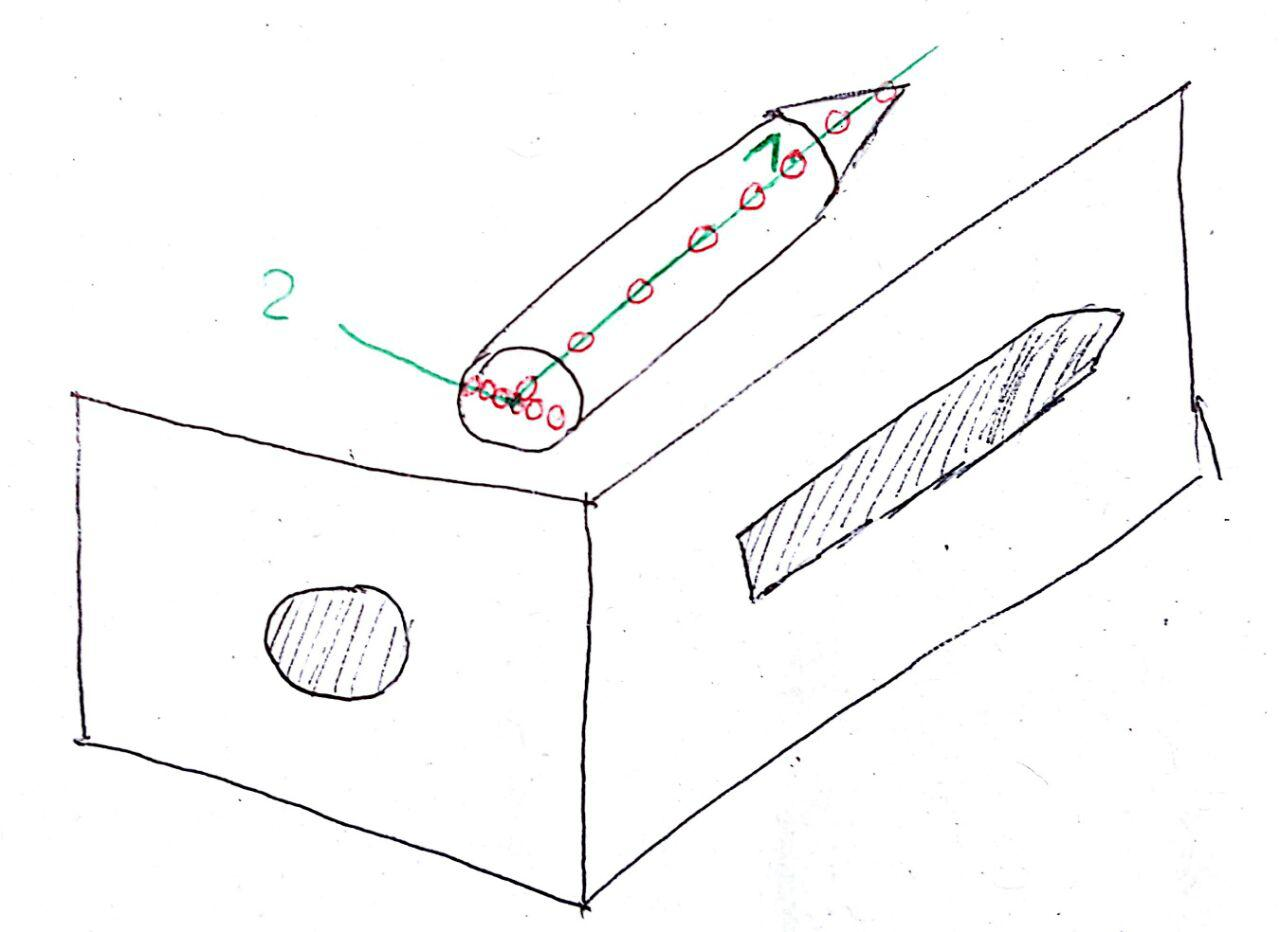
\includegraphics[width=0.5\linewidth]{tema_2/images/llapis.jpg}
	\caption{Representació projecció llapis}
	\label{fig:llapis}
\end{figure}

Podem escollir diversos plans on projectar el llapis. Si es fa una projecció en alçat es veurà el llapis estirat i segons com es projecti de perfil només es veurà un cercle.

Quina de les dues representacions és millor? Què volem? 
\begin{itemize}
	\item Representar les dades de la manera més fidel? (Representació en alçat)
	\item Representar les dades de la manera més reduïda possible? (Representació de perfil)
\end{itemize}

També es poden representar les dades sobre l'eix de revolució del llapis. O sobre un eix perpendicular a aquest. El que busquem és que les dades tinguin la màxima variabilitat possible.

\textbf{Formalització}: Tenim una mostra de dades $\{x_1, ..., x_n\}$ tal que $\bmath{x}_i \in \mathbb{R}^d$; provenen d'un vector aleatori $\bmath{X} = (X_1, ..., X_d)^T$ que té mitjana $\bmath{\mu} \in \mathbb{R}^d$ i una matriu de covariàncies $\Sigma = \left\{ \sigma_{ij}^2 \right\}$.

\begin{itemize}
	\item $\bmath{\mu} = \mathbb{E}(X) = \mathbb{E}(\bmath{X_1}, ..., \bmath{X_d})$
	\item $\Sigma = \frac{1}{N} \sum_{n=1}^N \left((\bmath{X}_n - \bmath{\mu})(\bmath{X}_n - \bmath{\mu})^T\right)$
	
	\begin{flalign*}
	\text{En particular } & CoVar(X_i, X_j) = \sigma_{ij}^2  &\\
 & CoVar(X_i, X_i) = \sigma_{ii}^2 = Var(X_i) =\sigma_i^2 &
	\end{flalign*}
\end{itemize}

Considerem el problema de trobar unes variables noves $Y = (Y_1, ..., Y_d)^T$ tal que:

\begin{enumerate}
	\item $CoVar(Y_i, Y_j) = 0$ per $i \ne j$
	\item $Var(Y_1) > Var(Y_2) > ... > Var(Y_d)$
	\item $\sum_{i=1}^d Var(X_i) = \sum_{i=1}^d Var(Y_i)$
\end{enumerate}

Busquem un \textbf{mètode lineal}: les $Y_j = a_j^TX, j=1,...,d$

Imposem una condició de \textbf{normalització} $||a_j||^2 = 1$ 
(Transformació \textbf{ortogonal})

\subsection{Tria de $a_1$}
Cal que $a_1$ maximitzi la $Var(Y_1)$ subjecte a $||a_1||^2=1$
$$ \op{Var}(Y_1) = \op{Var}(a_1^TX) = a_1^T \op{Var}(X)a_1 = a_1^T\Sigma a_1 $$

\textbf{Excursió}: multiplicadors de Lagrange

Sigui $f:\mathbb{R}^d \rightarrow \mathbb{R}$ diferenciable i la volem maximitzar subjecte a una \textbf{condició d'igualtat} $g(x_1, ..., x_d) = c$.

Una manera de fer-ho és construir el Lagrangià:

$$  
L(x) = f(x) - \lambda(g(x) - c)  
$$

La solució és un punt estacionari (les derivades s'anu\l.len).
$$  
\frac{\partial L}{\partial x_i} - \lambda \frac{\partial g}{\partial x_i} = 0, i = 1, ..., d \implies 
L(a_1) = a_1^T\Sigma a_1 - \lambda(||a||^2 - 1)  
$$

\begin{itemize}
	\item $\frac{\partial L}{\partial a_1} = 2\Sigma a_1 - 2\lambda a1 = 0$
	\item $\Sigma a_1 = \lambda a_1$
	
	$a_1$ és un vector propi de $\Sigma$ amb valor propi $\lambda$
	\item $Var(Y_1) = a_1^T\Sigma a_1=a_1^T(\lambda a_1) = \lambda(a_1^T a_1) = \lambda ||a_1||^2 = \lambda$
	
	\textbf{Mètode}: triem $\lambda$ on el VAP $\Sigma$ més gran
	
	$\lambda_1, ..., \lambda_d \implies \lambda_1 > \lambda_2 > ... > \lambda_d > 0$
\end{itemize}

\subsection{Tria de $a_2$}

$Y_2 = a_2^TX$ on $||a_2||^2 = 1$ i 
\begin{align*}
	& 
	\begin{aligned}
		CoVar(Y_2, Y_1) &= CoVar(a_2^TX, a_1^TX) = a_2^T\Sigma a_1 
		\underbrace{= 0}_{\mathclap{\text{es vol que sigui 0}}} \\
		& = a_2^T(\Sigma a_1) = a_2^T(\lambda_1 a_1) = \lambda_1 (a_2^Ta_1) 
		\underbrace{= 0}_{\mathclap{\text{es vol que ho sigui}}} \Leftrightarrow a_1 \bot a_2
	\end{aligned} \\
	& L(a_2) = a_2^T\Sigma a_2 - \lambda(||a_2||^2 - 1) - \delta(a_2^Ta_1) \implies \Sigma a_2 = \lambda a_2
\end{align*}

S'escull $a_2$ com el vector associat al segon VAP més gran de $\Sigma \rightarrow \lambda_2$

\subsection{Resultats}
\begin{enumerate}
	\item Si s'anomena $\Delta$ a la matriu de covariàncies de $Y$, és clar que
	$$
	\Delta = 
	\begin{pmatrix}
		 \lambda_1 &   &   & \text{\huge0 } \\
		 & \lambda_2 &   &  \\
		 &  & \ddots &  \\
		 \text{ \huge0} &  &  &  \lambda_d
	\end{pmatrix}
	$$
	
	donats: $a_3, ..., a_d$ es deriven igual els $a_1, ..., a_d$ i es diuen \textbf{components principals}.
	
	\item Per construcció
	\begin{flalign*}			
		& \overset{Var(Y_1)\ >}{\underset{\lambda_1}{\verteq}} 
		\overset{Var(Y_2)\ >}{\underset{\lambda_2}{\verteq}}
		\overset{...\ >\ Var(Y_d)}{\underset{\lambda_d}{\verteq}} &
	\end{flalign*}
 
	
	\item $\sum_{i=1}^d Var(Y_i) = \sum_{i=1}^d \lambda_i 
	\underbrace{=}_{\mathclap{\text{teorema}}} Tr(\Sigma) = 
	\sum_{i=1}^d \sigma_i^2 = \sum_{i=1}^d Var(X_i)$
\end{enumerate}

\textbf{Idea}: quedar-se amb els $k$ primers components principals $a_1, ..., a_k\ (k<d)$ (Per visualitzar $k=\{2,3\})$. Si decidim quedar-nos amb les $k$ primeres:

$$ 
\%\text{de variància retinguda } = \frac{\sum_{i=1}^k \lambda_i}{\sum_{i=1}^d \lambda_i}·100 
$$

% Formula 1 aquí

\textbf{Algorisme} PCA $(X, k = 2)$

\begin{itemize}
	\item Calcular la mitjana de les dades $\hat{\mu}$
	\item Centrar les dades $x_n \leftarrow x_n - \hat{\mu}, n = 1, ..., N$
	\item Calcular els VEPs i VAPs de $\hat{\Sigma}$
	
	ret $A \leftarrow (a_1, a_2, ..., a_k)$
\end{itemize}

\section{Anàlisi discriminant de Fisher}
$$  
\mathcal{D} = \{(x_1, t_1), ..., (x_N, t_N)\}, \boldsymbol{x_n \in \mathbb{R}^d}, t_n \in \{-1, +1 \}  
$$

% Figura 2

\textbf{Notació}
$$  
C_+, C_-  
$$
\begin{align*}
	C_+ &:= \{ n | t_n = +1 \} \\
	C_- &:= \{ n | t_n = -1 \} \\
	\bmath{m}_+ &:= \frac{1}{|C_+|} \sum_{n\in C_+} \bmath{x}_n \\
	\bmath{m}_- &:= \frac{1}{|C_-|} \sum_{n\in C_-} \bmath{x}_n \\
\end{align*}

Si es suposa que es té vector $D$-dimensional i es vol projectar a una dimensió s'està buscant un $w$ tal que $y_n = w^T \bmath{x}_n$. Així doncs, es busca un $w$ tal que maximitzi la separació entre les mitjanes projectades $m_+ - m_- = \bmath{w}^T(\bmath{m}_+ - \bmath{m}_-)$ on $m_k = w^T \bmath{m}_k$.

La \textbf{dispersió} (\emph{scatter}) d'una classe projectada:

$$  
s_+^2 := \sum_{n \in C_+} (y_n - m_+)^2 = 
\sum_{m \in C_+} (\bmath{w}^T \bmath{x}_n - \bmath{w}^T \bmath{m}_+)^2
$$
(és la variància, excepte la divisió per $|C_+| - 1$)

$s_-^2$ anàlogament 

$$
s_-^2 := \sum_{n \in C_-} (y_n - m_-)^2 = 
\sum_{m \in C_-} (\bmath{w}^T \bmath{x}_n - \bmath{w}^T \bmath{m}_-)^2
$$

La \textbf{dispersió total} és $s_+^2 + s_-^2$.

El criteri de Fisher és $$  J(\bmath{w}) = \underbrace{\frac{|\bmath{w}^T(\bmath{m}_+-\bmath{m}_-)|}{s_+^2 + s_-^2}}_\text{a maximitzar}  $$

La solució és $\bmath{w}^* = S_w^{-1}(\bmath{m}_- - \bmath{m}_+)$

$S_w$ és la matriu de dispersió intra-classe (\emph{within-class scatter matrix}):

$$
S_w = S_+ + S_- = 
\underbrace{\sum_{n \in C_+} (x_n - \bmath{m}_+)(x_n - \bmath{m}_+)^T}_{S_+} +
\underbrace{\sum_{n \in C_-} (x_n - \bmath{m}_-)(x_n - \bmath{m}_-)^T}_{S_-}  
$$


$S_B$ és la matriu de dispersió inter-classe (\emph{between-class scatter matrix}):
$$
S_B = (\bmath{m}_- - \bmath{m}_+)(\bmath{m}_- - \bmath{m}_+)^T
$$

\chapter{Mètodes de \emph{clustering}}
\textbf{Objectiu}: El nostre objectiu és trobar agrupacions naturals de dades. Un grup o subgrup de dades és un \emph{cluster}

Les observacions que pertanyen al mateix \emph{cluster} s'assemblen entre elles

Les observacions que \textbf{no} pertanyen al mateix \emph{cluster} no s'assemblen tant

\textbf{\emph{Clustering:}}
\begin{itemize}
	\item el \textbf{procés} de trobar els \emph{clusters} presents en les dades
	\item el \textbf{resultat} del procés.
\end{itemize}

\begin{figure}[h!]
    \centering
    \begin{minipage}[t]{0.49\textwidth}
        \centering
        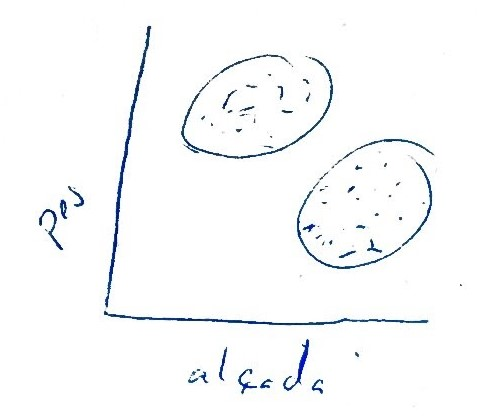
\includegraphics[width=\textwidth]{tema_3/images/figura_1}
        \caption{Diversos grups}
    \end{minipage}
    \hfill
    \begin{minipage}[t]{0.49\textwidth}
        \centering
        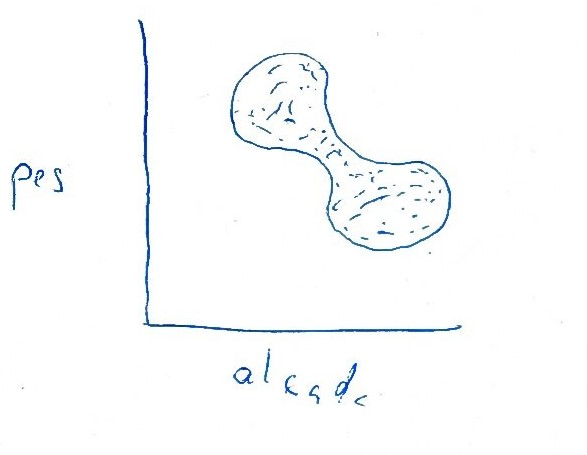
\includegraphics[width=\textwidth]{tema_3/images/figura_2}
        \caption{Agrupar mitjançant clustering}
    \end{minipage}
\end{figure}

\section{Mètodes de \emph{clustering}}

Un tipus de mètode són els mètodes jeràrquics:
\begin{itemize}
	\item \textbf{divisius} es dediquen a separar les dades en dos grups recursivament fins que només queda un punt.
	\item \textbf{aglomeratius} es dediquen a agrupar les dades des d'un punt fins a obtenir el \emph{cluster} final.
\end{itemize}

\begin{figure}[H]
    \centering
    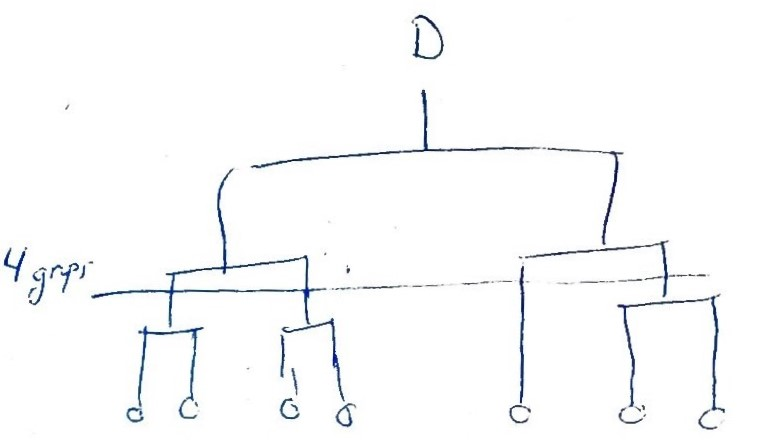
\includegraphics[width=0.5\textwidth]{tema_3/images/figura_3}
    \caption{Mètodes jeràrquics}
\end{figure}

També hi ha els mètodes combinatoris. Hi ha un algoritme voraç amb una funció de qualitat.

Hi ha els algoritmes probabilístics. De quantes maneres es poden agrupar $N$ dades en $K$ \emph{clusters}?

$$ 
S(N, K) = \frac{1}{K!} \sum_{k=1}^K (-1)^{K-k} 
\begin{pmatrix}
K \\ k
\end{pmatrix} 
\text{, nº d'Stirling del 2n tipus} \implies S(19,4) \simeq 10^{10} 
$$

$$ 
\underbrace{B(N)}_{\text{nº de Bell}} \sum_{K=1}^{N} S(N,K) \implies \text{ ex.: } B(79) \simeq 3.89·10^85 
$$

Així doncs hi ha diferents mètodes de \emph{clustering} per trobar els grups.

\section{Algorisme de $k$-means}

Tenim una mostra $\mathcal{D} = \{ x_1,..., x_N \} , x_i \in \mathbb{R}, 1 \le i \le N$. Fixa't $K$ externament, escollim un conjunt de $K$ \textbf{prototips}:

$$ \mathcal{P} = \{ \mu_1, ..., \mu_K \}, \mu \in \mathbb{R}^d $$

\begin{figure}[H]
    \centering
    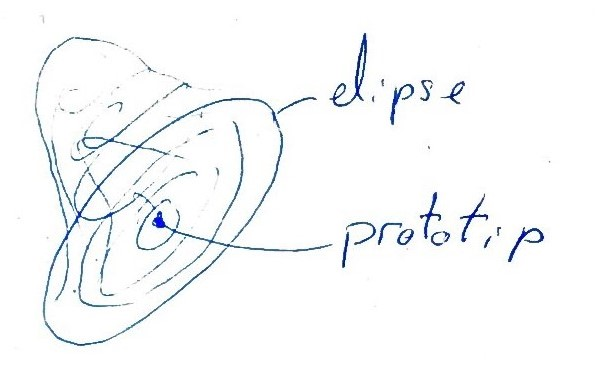
\includegraphics[width=0.5\textwidth]{tema_3/images/figura_4}
    \caption{Anells d'agrupacions gaussianes}
\end{figure}

\begin{itemize}
	\item El nostre objectiu és trobar un conjunt de prototips $\mathcal{P}$ tal que les dades de $\mathcal{D}$ que estiguin assignades al \emph{cluster} $k$ es trobin més a prop de $\mu_k$ que de cap altre.
	\item Definim les variables indicadores:
	
	$$ 
	r_{nk} =
	\begin{cases}
	1 & \text{si } k = argmin ||x_n - \mu_j||\ 1 \le j \le K \\ 0 & \text{en cas contrari}
	\end{cases}
	$$
	
	\item Definim un criteri de qualitat, a minimitzar, tenint en compte que minimitzar la distància al quadrat és el mateix que minimitzar la distància:
	
	$$ J(\mathcal{P}, \{r_{nk}\}) = \sum_{n=1}^N \sum_{k=1}^K r_{nk} ||x_n - \mu_k||^2 $$
	
	\begin{itemize}
		\item Si sapiguessim la solució per $\mathcal{P}$, com trobaríem la solució pells $\{r_{nk}\}$? Calculant les distàncies als $\mathcal{P}$.
		
		\item Si sapiguessim la solució per $\{r_{nk}\}$ com trobaríem la solució per $\mathcal{P}$? El prototip òptim és el centroide (la mitjana) de les dades assignades a cada \emph{cluster}.
	\end{itemize}
\end{itemize}

\subsection{Formalització}
\begin{itemize}
	\item Donat $\mathcal{P} = \{ \mu_1, ..., \mu_K \}$ recalcular els $\{r_{nk}\}$
	
	$$ r_{nk} =
	\begin{cases}
	1 & \text{si } k = argmin ||x_n - \mu_j||\ 1 \le j \le K \\ 0 & \text{en cas contrari}
	\end{cases}$$
	
	\item Recalcular $\mathcal{P}$ a partir dels $\{r_{nk}\}$
	
	\begin{itemize}
		\item $\frac{\partial J}{\partial \mu_k} = \sum_{n=1}^N r_{nk} \underbrace{\frac{\partial ||x_n - \mu_k||^2}{\partial \mu_k}}_{-2(x_n - \mu_k)} = 2\sum_{n=1}^N r_{nk} (\mu_k - x_n) = 0$
		
		$\sum_{n=1}^N r_{nk}\mu_k = \sum_{n=1}^N r_{nk}x_n \implies \mu_k\sum_{n=1}^N r_{nk} = \sum_{n=1}^N r_{nk}x_n \implies \boxed{\mu_k = \frac{\sum_{n=1}^N r_{nk}}{\sum_{n=1}^N r_{nk}}}$
		
		\item Tenint en compte que $\frac{\partial ||\vec{z}||^2}{\partial \vec{z}} = \begin{pmatrix}
		2z_1 \\ 2z_2 \\ \vdots \\ 2z_d
		\end{pmatrix} = 2\vec{z}$
	\end{itemize}
\end{itemize}

\subsection{Algorisme}

\begin{algorithmic}
    \State Inicialitzar $\mathcal{P}$
    \While{no convergeixi}
        \State Recalcular els $r_{nk}$ usant $\mathcal{P}$
        \State Recalcular $\mathcal{P}$ usant els $r_{nk}$
    \EndWhile
    \State \Return $\mathcal{P},r_{nk}$
\end{algorithmic}


\subsection{Comentaris}

\begin{enumerate}
	\item $\Downarrow$ Cal una inicialització de $\mathcal{P}$, que és un problema en sí mateix
	\item $\Downarrow$ L'assignació de dades als \emph{clusters} $\{r_{nk}\}$ és \textbf{binària} per tant és difícil.
	\item $\Downarrow$ Cal un procediment extern de determinació de $K$.
\end{enumerate}

\section{Barreges de Gaussianes (Mixture of Gaussians)}

Determinació de \textbf{funcions de densitat de probabilitat (pdf)}. Tenim una mostra de dades  $\{x_1,...,x_n\}$ i.i.d (simple) generar una pdf $p(x)$. Això és impossible a no ser que reduïm les possibilitats.

El que farem serà agafar unes quantes gaussianes i comprovar quin percentatge de la solució final representen.

\begin{figure}[H]
    \centering
    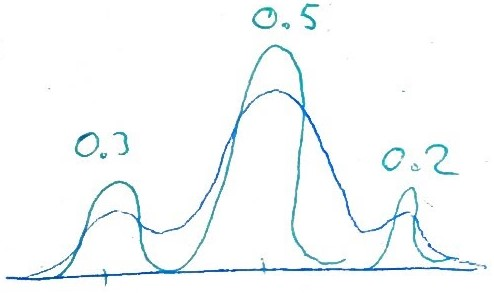
\includegraphics[width=0.5\textwidth]{tema_3/images/figura_5}
    \caption{Barreja de Gaussianes}
\end{figure}

En dues dimensions es tenen unes dades podem trobar uns conjunts de gaussianes, es solaparan perquè les gaussianes tenen amplada infinit. Un cop trobades les ponderem i busquem la densitat final.

\begin{figure}[H]
    \centering
    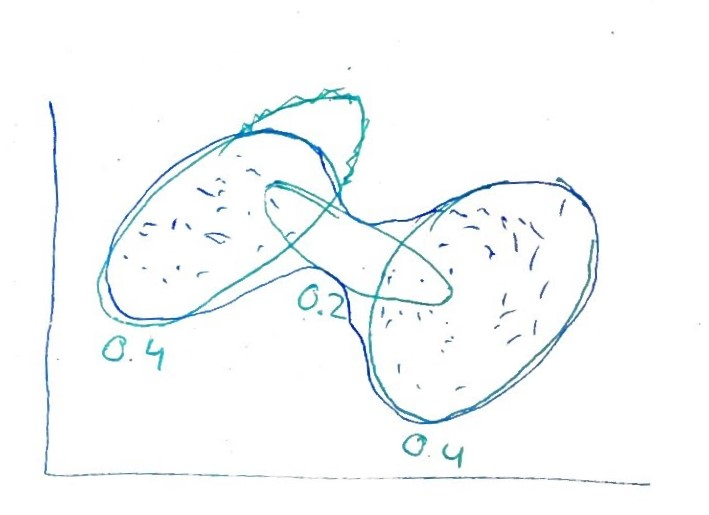
\includegraphics[width=0.5\textwidth]{tema_3/images/figura_6}
    \caption{Diverses agrupacions Gaussianes}
\end{figure}

Una barreja de Gaussianes és una pdf de la forma:

$$ 
p(x) = \sum_{k=1}^K \underbrace{\pi_k}_{\text{Coeficients}}·
\underbrace{N(x, \mu_k, \Sigma_k)}_{\text{Components de la barreja}}, 
0 \le \pi_k \le 1, \sum_{k=1}^K \pi_k = 1
$$

\begin{align*}
	\{\pi_k, \mu_k, \Sigma_k\} & \text{  desconegudes, paràmetres} \\
	K & \text{  desconegudea (hiper-paràmetre)}
\end{align*}

A vegades generalitzar el problema ajudar a trobar solucions que a simple vista no es poden veure per casos particulars. 

En principi la distribució $p$ només pertany de les variables $x$. Creem una nova variable aleatòria $z$ que ens ajuda a veure el problema de manera més general.

$$
p(\underbrace{x}_{x \in \mathbb{R}^d}) \to p(x,z) = p(x|z)·p(z)
$$

$$ 
z = 
\begin{pmatrix}
z1 \\ \vdots \\ z_K
\end{pmatrix} \text{Només una component de z és 1} 
$$

$$
z = 
\begin{pmatrix}
0 \\
0 \\
1 \\
0 \\
0
\end{pmatrix}
\to
\parbox{14em}{La $x$ associada a $z$ ha estat generada per la componen $k=3$ (amb probabilitat $\pi_3$)}
$$

S'interpreta com que ha estat la coponent $k$ la que ha generat X. Aquestes $z$ s'anomenen \textbf{variables aleatòries latents o ocultes}.

\begin{description}
	\item[Distribució marginal sobre z] $p(z_k = 1) = \pi_k$
	
	$p(z) = \prod_{k=1}^K {\pi_k}^{z_k}$
	
	\item[Distribució condicional] de $x$ respecte $z$
	
	$p(x|z_k = 1) = N(x, \mu_k, \Sigma_k)$
	
	\item[Distribució marginal sobre $x$] ara eliminem la $z$
	
	$p(x) = \sum_z p(x|z)p(z) = \sum_{k=1}^K \pi_k N(x, \mu_k, \Sigma_k)$
	
	\item[Distribució condicional] de $z$ respecte $x$
	
	$p(z_k = 1|x) = \frac{p(x|z_k = 1)p(z_k = 1)}{p(x)} = 
	\frac{N(x, \mu_k, \Sigma_k)·\pi_k}{\sum_{j=1}^K \pi_j · N(x, \mu_j, \Sigma_j)}$
	
	$\gamma_k(x) := p(z_k = 1 | x) \to \parbox{14em}{Probabilitat de que $x$ hagi estat generada per la component $k$ }$
	
	$\pi_k \to$ Prioritat a priori
	
	$p(z_k = 1 | x) \to$ Prioritat a posteriori
\end{description}

\subsection{Problema d'estimació de paràmetres: $\{\pi_k\}, \{ \mu_k \}, \{ \Sigma_k \}$ }

\subsubsection{Màxima versemblança}

$$ \{\pi_k\}, \{ \mu_k \}, \{ \Sigma_k \} = \theta $$
\begin{align*}
	\ell(\theta) &= ln \mathcal{L}(\theta) = ln P(\mathcal{D}|\theta) =
	ln \prod_{n=1}^N P(x_n | \{\pi_k, \mu_k, \Sigma_k \}) = \\
	&= ln \prod_{n=1}^N \sum_{k=1}^K \pi_k N(x_n, \mu_k, \Sigma_k) = 
	\sum_{n=1}^N ln\left(\sum_{k=1}^K \pi_k N\left(x_n, \mu_k, \Sigma_k \right) \right)
\end{align*}

$$
N(x, \mu, \Sigma) = \underbrace{|\Sigma|^{-\frac{1}{2}}·(2\pi)^{-\frac{d}{2}}}_C·exp\left( -\frac{1}{2}(x - \mu)^T \Sigma^{-1}(x-\mu) \right)
$$

\begin{flalign*}
	\textbullet &\frac{\partial \ell(\theta)}{\partial \mu_k} &&= \sum_{n=1}^N 
	\frac{1}{\sum_{j=1}^K \pi_j · N(x_n, \mu_j, \Sigma_j)}·\pi_k · 
	\frac{\partial N(x_n, \mu_k, \Sigma_k}{\partial \mu_k} =  && \\
	& &&= \sum_{n=1}^N 
	\underbrace{
		\frac{\pi_k·N(x_n, \mu_k, \Sigma_k)}{\sum_{j=1}^K \pi_j · N(x_n, \mu_j, \Sigma_j)}
	}_{\gamma_k(x_n)} \Sigma_k^{-1} (x_n - \mu_k) = \\
	& && = \sum_{n=1}^N \gamma_k (x_n) · \Sigma_k^{-1} (x_n - \mu_k) = 0 \implies \\
	& && \implies \sum_{n=1}^N \gamma_k (x_n) · \Sigma_k^{-1} x_n = 
	\sum_{n=1}^N \gamma_k(x_n) · \Sigma_k^{-1} \mu_k \implies \\
	& &&  \implies \cancel{\Sigma_k^{-1}} \left(\sum_{n=1}^N \gamma_k(x_n)·x_n \right) = \cancel{\Sigma_k^{-1}} \mu_k \left( \sigma_{n=1}^N \gamma_k(x_n) \right) \implies \\
	& && \implies 
	\boxed{\mu_k = \frac{\sum_{n=1}^N \gamma_k (x_n) · x_n}{\sum_{n=1}^N \gamma_k(x_n)}} 
\end{flalign*}
\begin{flalign*}
	\textbullet &\frac{\partial N(x, \mu, \Sigma}{\partial \mu} &&= 
	C\exp\left( -\frac{1}{2}(x - \mu)^T \Sigma^{-1}(x-\mu) \right)
	\cancel{\frac{-1}{2}}
	\underbrace{\frac{\partial \left\{ (x - \mu)^T \Sigma^{-1} (x - \mu) \right\} }{\partial \mu}}_{\cancel{-2}\Sigma^{-1}(x-\mu)} = \\ 
	& && = N(x,\mu,\Sigma)\Sigma^{-1}(x-\mu) &&
\end{flalign*}
\begin{flalign*}
	&\textbullet \frac{\partial z^T A z}{\partial z} = 
	(A + A^T) z \underbrace{=}_{\mathclap{\parbox{3em}{\tiny Si A és simètrica}}} 2Az &&
\end{flalign*}
\begin{flalign*}
	\textbullet\frac{\partial \ell(\theta)}{\partial \Sigma_k} = 0 \implies 
	\boxed{\Sigma_k = \frac{\sum_{n=1}^N \gamma_k(x_n) (x_n - \mu_k)(x_n - \mu_k)^T}{\sum_{n=1}^N \gamma_k (x_n)}}
	&&
\end{flalign*}

\begin{flalign*}
	\textbullet &\sum_{n=1}^K \pi_k = 1 \implies mcx\ \ell(\theta) + \lambda·\left( \sum_{k=1}^K \pi_k - 1 \right) \\
	& \frac{\partial \ell(\theta)}{\partial \pi_k} =
	\sum_{n=1}^N \frac{1}{\sum_{j=1}^K \pi_j·N(x_n,\mu_j, \Sigma_j)}·N(x_n,\mu_k,\Sigma_k) + \lambda = 0
	\underset{\times\pi_k}{\implies} \\
	& \underset{\times\pi_k}{\implies}
	\underset{\forall k, 1 \le k \le K}{\sum_{n=1}^N \gamma_k(x_n) + \lambda \pi_k = 0} \implies 
	\sum_{k=1}^K \sum_{n=1}^N \gamma_k(x_n) + \lambda \underbrace{\sum_{k=1}^K \pi_k}_1 = 0 \implies
	\\
	& \implies \sum_{n=1}^N \underbrace{\sum_{k=1}^K \gamma_k(x_n)}_1 + \lambda = 0 \implies N + \lambda = 0 \implies \boxed{\lambda = -N} &&
\end{flalign*}

$$
\boxed{\pi_k = \frac{1}{N} \sum_{n=1}^N \gamma_k(x_n)}
$$

\subsubsection{Algorisme E-M Moos $(\mathcal{D},K)$}

Aquest algoritme serveix en general per maximitzar una funció de versemblança complexa.

\begin{algorithmic}
	\State Inicialitzar $ \{ \pi_k, \Sigma_k, \mu_k, \quad 1 \le k \le K \} $
	\State 
	$
	k-means(\mathcal{D},K) \circlearrowleft \to 
	\begin{cases}
		\mu_k \\
		\{ r_{nk} \} 
		\begin{cases}
			\Sigma_k \\
			\pi_k
		\end{cases}
	\end{cases}
	$
	\Repeat 
		\State Calcular $\gamma_k(x_n), \forall k, \forall n \leftarrow$ calcular els \textbf{valors esperats} de les probabilitats a posteriori $\gamma_k (x_n)$
		\State Calcular les $ \{ \pi_k, \mu_k, \Sigma_k \},\ \forall k \leftarrow $ calcular per \textbf{maximització directa} (par M)
	\Until{convergeixi}
\end{algorithmic}

\documentclass[a4paper]{article}

\usepackage{amsmath}
\usepackage{amssymb}
\usepackage{amsfonts}
\usepackage[catalan]{babel} % Language 
\usepackage{fontspec}
\usepackage[margin=2cm]{geometry}
\usepackage{graphicx}
\usepackage[makeroom]{cancel}
\usepackage{float}

\setlength{\parindent}{0pt}
\setlength{\parskip}{0.2cm}

\title{Tema 4: Models lineals per regressió}
\author{Joan Marcè Iguals}

\begin{document}
\maketitle

\section{Introducció}
El problema de la regressió consisteix en, donat un vector $x \in \mathbb{R}^d$, predir un escalar $t \in \mathbb{R}$, on la relació (la dependència) entre $t$ i $x$ és estocàstica, així doncs escrivim:


\begin{align*}
t = f(x) + \varepsilon,\ \varepsilon &\text{ variable aleatòria} \\
i) \quad &\mathbb{E}(\varepsilon) = 0 \\
ii)\quad & Var(\varepsilon) = \sigma^2 < \infty
\end{align*}

Veiem unes dades:

$$
\mathcal{D} = \{ (x_1, t_1), ... (x_n, t_n)  \} \quad x_n \in R^d, t_n \in R^d \quad m.a.s.
$$

\textbf{Exemple:} ajust polinòmic

$$
y(x, c) = co + \sum_{i=1}^M c_i x^i \quad x \in \mathbb{R}
$$
$$
x \in \mathbb{R}^d\ ? \text{ els polinomis \textbf{no escalen} a més d'una variable}
$$

Introduïm el concepte de \textbf{funcions de base}

$$
\phi_i: \mathbb{R}^d \rightarrow \mathbb{R}, \quad i = 1,...,M
$$
\begin{align*}
y(x, \omega) &= \omega_0 + \sum_{i=1}^{M-1} \omega_i \phi_i (x) \\
&=  \sum_{i=0}^{M-1} \omega_i \phi_i (x), \quad \phi_0 (x) = 1
\end{align*}
\textbf{Exemple:} $\phi_i (x) = x^i$

Escrivim
$$
y(x, \omega) = \sum_{i=0}^{M-1} \omega_i \phi_i (x) = \vec{\omega}^T \vec{\phi} (x)
$$

$$
\vec{\omega} = 
\begin{pmatrix}
\omega_0 \\ \omega_1 \\ \vdots \\ \omega_{M-1}
\end{pmatrix};\quad
\vec{\phi}(x) = 
\begin{pmatrix}
\phi_0 (x) = 1 \\
\phi_1 (x) \\
\vdots \\
\phi_{M-1}
\end{pmatrix}
$$

\section{Regressió clàssica}

$$
\varepsilon ~ N(0, \sigma^2)
$$

Si tenim una distribució normal (veure figura 1) l'amplada del pic de la gaussiana depèn de $\sigma^2$.


% FIGURA 1

$ t = f(x) + N(0, \sigma^2) $ és equivalent a escriure $T ~ N(f(x), \sigma^2) $.

Així doncs si s'agafa la mitjana de $x$ i s'uneixen els punts, la funció resultant és la millor possible. Així doncs la funció de regressió $f^*(x) = \mathbb{E}(T|X)$.

L'únic que ens falta és posar les dades en una matriu:

$$
\vec{X}_{N \times d} =
\begin{pmatrix}
\leftarrow x_1 \rightarrow \\
\leftarrow x_2 \rightarrow \\
\vdots \\
\leftarrow x_N \rightarrow
\end{pmatrix}
$$

Així doncs tenim $\mathcal{D}$ conegudes $(x_n, t_n)$, $\omega$ i $\sigma^2$ desconeguts, per tant apliquem \textbf{Màxima Versemblança}.

$$
\theta = (\omega, \sigma^2)
$$

\begin{align*}
-\ell (\theta) &= -ln \mathcal{L} (\theta) = 
-ln \mathcal{\omega, \sigma^2} =
-ln P(t | X, \omega, \sigma^2) \underbrace{=}_{m.a.s.} \\
-ln \prod_{n=1}^N P(t_n | x_n, \omega, \sigma^2) &\underbrace{=}_{modelat}
-ln \prod_{n=1}^N \mathcal{N} (t_n, y(x_n, \omega), \sigma^2) =
- \sum_{n=1}^N ln \ \mathcal{N} (t_n, y(x_n, \omega), \sigma^2) = \\
- \sum_{n=1}^N \left\{ ln \left( \frac{1}{\sqrt{2\pi}\sigma} \right) - \frac{(t_n - y(x_n, \omega))^2}{2\sigma^2} \right\} &= 
\sum_{n=1}^N \left\{ ln(\sqrt{2\pi}\sigma) + \frac{(t_n - y(x_n, \omega))^2}{2\sigma^2} \right\} = \\
N ln (\sqrt{2\pi}) + \frac{1}{2\sigma^2} \sum_{n=1}^N (t_n - y(x_n,\omega))^2 & \text{ és equivalent a } \frac{1}{2} \sum_{n=1}^N (t_n - y(x_n, \omega))^2 = E(\omega)
\end{align*}

$$
\boxed{y(x, \omega) = \omega^T \phi(x)} \text{ és convinent }
$$

$$
\Phi_{N \times M} =
\begin{pmatrix}
\phi_0 (x_1) & \phi_1(x_1) & \ldots & \phi_{M-1} (x_1) \\
\phi_0 (x_2) & \phi_1(x_2) & \ldots & \phi_{M-1} (x_2) \\
\vdots & \vdots & \ddots & \vdots \\
\phi_0 (x_N) & \phi_1(x_N) & \ldots & \phi_{M-1} (x_N)
\end{pmatrix}
\text{ matriu de disseny}
$$

$$
\mathcal{N}(t, \mu, \sigma^2) = \frac{1}{\sqrt{2 \pi} \sigma} exp \left( - \frac{(t - \mu)^2}{2\sigma^2} \right)
$$

Expressem \textbf{l'error quadràtic}
$$
E(\omega) = \frac{1}{2} || \vec{t} - \Phi \vec{\omega} ||^2 = \frac{1}{2} \left\{ ||\vec{t}||^2 + ||\Phi \vec{\omega}||^2 - 2t^T(\Phi \vec{\omega}) \right\}
$$

$$
\frac{\partial E}{\partial \vec{\omega}} = \frac{1}{2} \left\{ 0 + 2 \Phi^T \Phi \hat{\vec{\omega}} - 2 \Phi^T \vec{t} \right\} = \Phi^T \Phi \hat{\vec{\omega}} - \Phi^T \vec{t} = \vec{0} \implies
$$
$$
\left( \Phi^T \Phi \right) \hat{\vec{\omega}} = \Phi^T \vec{t} \implies
\boxed{\hat{\vec{\omega}} = (\Phi^T \Phi)^{-1} \Phi \vec{t}} = \Phi^+ \vec{t}
$$
$$
\frac{\partial E}{\partial \sigma^2} = \frac{1}{N} \sum_{n=1}^N (t_n - \vec{\omega}^T \phi(x_n))^2 = \frac{2}{N} E(\omega)
$$

\textbf{Teorema} ("mínims quadrats")
Sigui $\Phi_{N\times M}, \quad N > M$. Si els vectors columna de $\Phi$ són linealment independents, és a dir, $rang(\Phi) = M$ (\emph{full rank}), llavors:

\begin{enumerate}
	\item La matriu $\Phi^T\Phi$ és simètrica i semi-definida positiva
	\item El problema de mínims quadrats: 
	$\underset{\vec{\omega}}{min} ||\vec{t} - \Phi \vec{\omega}||^2$ té solució única.
	\item Per trobar-la, cal resoldre el sistema d'equacions: $\Phi^T\Phi \vec{\omega} = \Phi^T \vec{t}$ (equacions normals de'n Gauss)
\end{enumerate}

La matriu $ \Phi^+ := \left( \Phi^T \Phi \right)^{-1} \Phi^T $ és pseudo-inversa (inversa de Moore-Penrose) $ \Phi^+ \Phi = I $

\end{document}
\chapter{Classificadors generatius}
\section{Introducció}

Un \textbf{classificador} és una funció:
$$
y:\mathbb{R}^d \rightarrow \{ 1,2,...,K \}
$$
$$
K = 2 \rightarrow \text{classificació binària}
$$

Ens interessarà molt trobar mètodes que ofereixin probabilitats. Per exemple:
\begin{align*}
	K = 3 \qquad &x \rightarrow y(x) = "2" \quad (0\ 1\ 0) \quad \text{\textbf{HARD}}\\
	& x \rightarrow y(x) = (0.2, 0.5, 0.3) \quad \text{\textbf{SOFT}}
\end{align*}

Un classificador parteix $\mathbb{R}^d$ en $K$ subconjunts. 

\textbf{Regions de decisió:}

\begin{figure}[H]
	\centering
	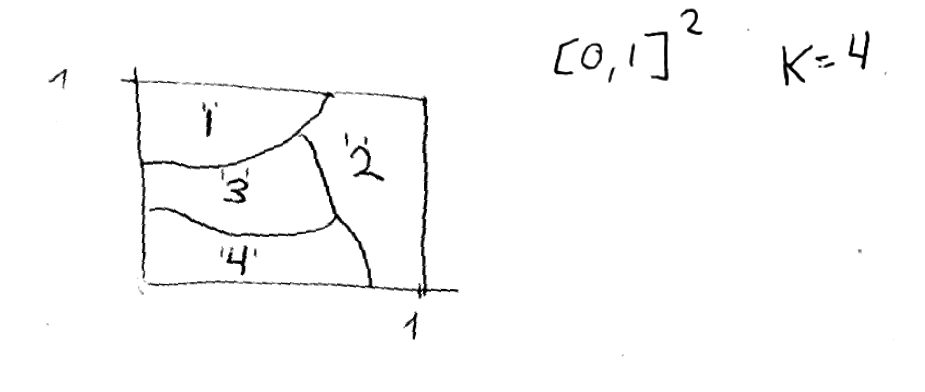
\includegraphics[width=0.5\textwidth]{tema_5/images/tema_5-1}
\end{figure}

Les regions de decisió estan generades per les zones que delimiten cada classe. Hi ha unes fronteres on les regions canvien. Les separacions es diuen \emph{fronteres de decisió}.

Un classificador és \textbf{lineal} quan només genera fronteres de decisió (entre cada parell de classes) lineals. Per exemple:

\begin{figure}[H]
	\centering
	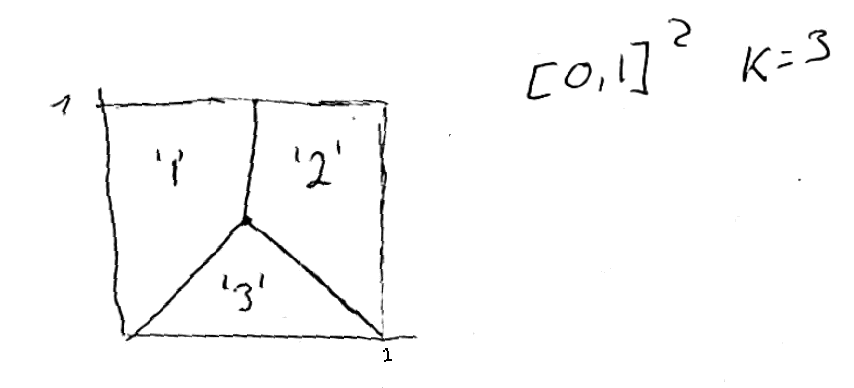
\includegraphics[width=0.5\textwidth]{tema_5/images/tema_5-2}
\end{figure}

\subsection{La formula de'n Bayes}

Suposem que tenim dues variables aleatòries $A$, $B$, que prenen valors en:

$$
\{ a_1, ..., a_n \}\quad \{ b_1, ..., b_n \}
$$
$$
\begin{cases}
p(a_k) = \sum_{j=1}^n P(a_k, b_j) = \sum_{j=1}^n P(a_k | b_j) P(b_j) \\
P(a_k, b_j) = P(b_j, a_k)
\end{cases}
$$
$$
P(a_k | b_j) P(b_j) = P(b_j | a_k) P(a_k) \implies
\boxed{P(b_j | a_k) = \frac{P(a_k | b_j) P(b_j)}{\sum_{q=1}^n P(a_k | b_q) P(b_q)}}
$$
$$
\sum_{j=1}^m P(b_j | a_k) = 1,\ \forall k 
$$

\textbf{Exemple:} Tenim dues urnes amb pomes ($P$) i taronges ($T$). La probabilitat d'agafar la urna 1 és $\frac{2}{3}$ i la d'agafar la urna 2 és de $\frac{1}{3}$. S'agafa d'una urna a l'atzar un a taronja, quina és la probabilitat que la taronja provingui de la urna 1?

$$
P(U_1|T) =  \frac{P(T|U_1) P(U_1)}{\underbrace{P(T|U_1)P(U_1) + P(T|U_2)P(U_2)}_{P(T)}} =
\frac{\frac{2}{7} · \frac{2}{3}}{\frac{2}{7}·\frac{2}{3} + \frac{7}{9}·\frac{1}{3}} =
\frac{36}{85} < \frac{1}{2}
$$

\begin{figure}[H]
	\centering
	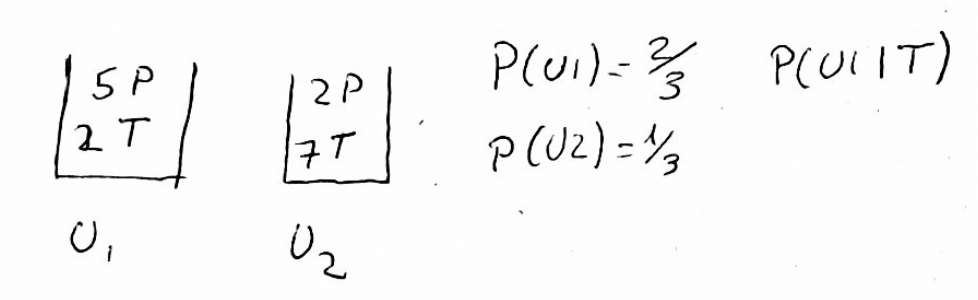
\includegraphics[width=0.7\textwidth]{tema_5/images/tema_5-3}
\end{figure}

\textbf{Exemple introductori:} Imaginem que tenim un amic ornitòleg que pren mesures de dos tipus d'aus \emph{àligues} i \emph{falcons} i pren mesures de la envergadura (en cm). El nostre amic vol decidir si a partir de la envergadura una au és una àliga o un falcó. 

\begin{figure}[H]
	\centering
	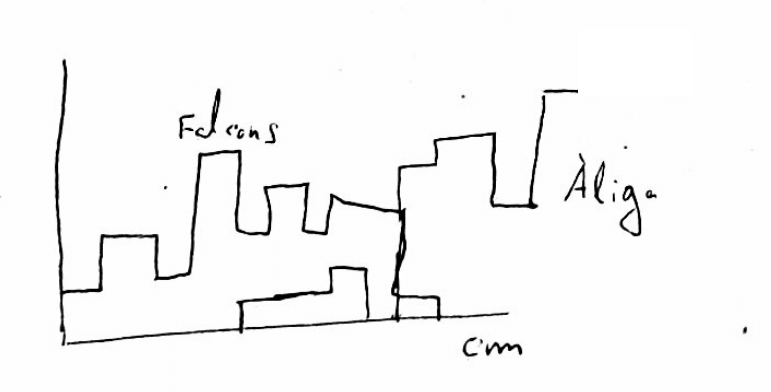
\includegraphics[width=0.7\textwidth]{tema_5/images/tema_5-4}
\end{figure}

Es tracta de donar una resposta que sigui la òptima. 
$$
N \text{ dades: }
\begin{rcases*}
N_1 \text{ falcons} \\
N_2 \text{ àligues}
\end{rcases*}
\begin{aligned}
C_1 \text{ (falcons)} \\
C_2 \text{ (àligues)}
\end{aligned}
$$

La mida de cada au no és estàndard sinó que varia en funció de l'entorn de manera aleatòria. 

$$
R_1: \text{ la classe de } x = 
\begin{cases}
C_1 \text{ si } \frac{N_1}{N} > \frac{N_2}{N} \\
C_2 \text{ si } \frac{N_2}{N} < \frac{N_1}{N}
\end{cases}
$$ 
Aquesta regla té força errors perquè és constant i no té en compte l'envergadura que hem estat mesurant.

$$
P_{R_1} (error) = \min\left(\frac{N_1}{N}, \frac{N_2}{N}\right) = \frac{1}{N} \min(N_1, N_2)
$$
$$
P_{R_2} (error) = \min(P(C_1), P(C_2))
$$
\begin{align*}
	& P(C_1 | X) = \frac{P(X|C_1)P(C_1)}{P(X|C_1)P(C_1) + P(X|C_2)P(C_2)} \\
	& P(C_2|X) = 1 - P(C_1|X)
\end{align*}

$$
R_{Bayes}: \text{ la classe de } X =
\begin{cases}
C_1 \text{ si } P(C_1|X) > P(C_2|X) \\
C_2 \text{ si } P(C_1|X) < P(C_2|X) \\
\end{cases}
$$
\begin{align*}
&P_{R_{Bays}} (error|X) = min\{P(C_1|X), P(C_2|X)\} \\
&P(error_{total}) = \mathbb{E}(P_{Bayes} (error|X)) = 
\int_{\mathbb{R}} P_{R_{Bays}} (error|X)P(X)dX =
\end{align*}
$$
\int_{\mathbb{R}} \min\{P(C_1|X),P(C_2|X)\}P(X)dX =
$$
$$
\int_{S} \min\left\{\frac{P(X|C_1)P(C_1)}{\cancel{P(X)}}, \frac{P(X|C_2)P(C_2)}{\cancel{P(X)}}\right\}\cancel{P(X)} dX \quad S = \{X|P(X) > 0\} =
$$
$$
\int_S \min\{ P(X|C_1)P(C_1), P(X|C_2)P(C_2) \} dX \le
$$
$$
\min\left\{ \int_S P(X|C_1)P(C_1) dX,\ \int_S P(X|C_2)P(C_2)dX \right\} =
$$
$$
\min\left\{ P(C_1)\int_S P(X|C_1)dX,\ P(C_2)\int_S P(X|C_2)dX \right\} =
$$
$$
\min \{ P(C_1), P(C_2) \} = P_{R_2} (error)
$$

$$
\int_S \min(f_1(x), f_2(x)) dx \le \min\left( \int_S f_1(x) dx,\ \int_S f_2(x) dx \right)
$$

\textbf{Teorema:} La $R_{Bays}$ és la millor regla de decisió (classificació) d'entre les que fan servir $P(C_1|X), P(C_2|X)$.



\begin{figure}[H]
	\centering
	\begin{tikzpicture}
		\pgfdeclarepatternformonly{flexible hatch}%
		{\pgfqpoint{-1pt}{-1pt}}%
		{\pgfqpoint{10pt}{10pt}}%
		{\pgfqpoint{6pt}{6pt}}%
		{
			\pgfsetlinewidth{1pt}
			\pgfpathmoveto{\pgfqpoint{6.1pt}{0pt}}
			\pgfpathlineto{\pgfqpoint{0pt}{6.1pt}}
			\pgfusepath{stroke}
		}
		\pgfdeclarepatternformonly{flexible inverted}%
		{\pgfqpoint{-1pt}{-1pt}}%
		{\pgfqpoint{10pt}{10pt}}%
		{\pgfqpoint{6pt}{6pt}}%
		{
			\pgfsetlinewidth{1pt}
			\pgfpathmoveto{\pgfqpoint{0pt}{0pt}}
			\pgfpathlineto{\pgfqpoint{6.1pt}{6.1pt}}
			\pgfusepath{stroke}
		}
		\begin{axis}[
				width=0.7\textwidth,height=0.7\textwidth,
				xmin=0,xmax=2.1,ymin=0,ymax=1.1,
				domain=0:2,
				axis x line=center,
				axis y line=center,
				axis on top,
				samples = 200,
				legend cell align = left,
				legend style={at={(0.9,0.5)},anchor=east},
			]
			\addplot+[black, mark=none, dashed, very thick]{max((2*x)/(x + 2),(2 - x)/(x + 2))};
			\addplot[mark=none, forget plot, black, dashed] coordinates {(2/3,0)(2/3,2)};
			\addplot[white, mark = none, area legend, pattern = flexible hatch, 
				pattern color = black!20!green!40] {1/3} \closedcycle;
			\addplot[white, mark=none, area legend, pattern = flexible inverted, 
				pattern color = orange!40] {min((2*x)/(x + 2),(2 - x)/(x + 2))} \closedcycle;
			\addplot[mark=none, orange]{1/3};
			\addplot[mark=none, purple]{2/3};
			\addplot[mark=none, red] {(2 - x)/(x + 2)};
			\addplot[mark=none, blue] {(2*x)/(x + 2)};
			\legend{$R_{bayes}$, $ \mathbb{E}(P_{error}(R_1))$,  $\mathbb{E}(P_{error}(R_{bayes}))$, 
				$P(C_1)$,$P(C_2)$, $P(C_1|X)$, $P(C_2|X)$};
		\end{axis}
	\end{tikzpicture}
	\caption{Gràfic amb la regla per classificar en funció del color i la probabilitat d'error}
	\label{fig:regla}
\end{figure}

\section{Classificadors generatius}

$$
P(C_1|X) = \frac{P(X|C_1)P(C_1)}{P(X|C_1)P(C_1) + P(X|C_2)P(C_2)} = 
\frac{1}{1 + \frac{P(X|C_2)P(C_2)}{P(X|C_1)P(C_1)}} =
$$
$$
\text{definim } a(x) := \ln \left( \frac{P(X|C_1)P(C_1)}{P(X|C_2)P(C_2)} \right)
$$
$$
P(C_1|X) = \frac{1}{1 + \exp(-a(x))} = 
$$
$$
\text{definim } g(z) := \frac{1}{1 + e^{-z}} \implies P(C_1|X) = g(a(x))
$$


\subsection{Funció logística}

$$
g:\mathbb{R} \rightarrow (0,1)
$$
La funció logística envia tots els valors de $\mathbb{R}$ a un valor comprès entre 0 i 1. Veure \autoref{fig:logistic}

\begin{figure}[H]
	\centering
	\begin{tikzpicture}
	\begin{axis}[
	xmin=-7,xmax=7,ymin=0,ymax=1,
	domain=-10:10
	]
	\addplot+[mark=none] {1/(1 + exp(-x))};
	\end{axis}
	\end{tikzpicture}
	\caption{Gràfic funció logística}
	\label{fig:logistic}
\end{figure}

\begin{itemize}
	\item $ \lim\limits_{z \to +\infty} g(z) = 1 $
	\item $ \lim\limits_{z \to -\infty} g(z) = 0 $
	\item $ g(-z) = 1 - g(z) $
	\item $ g(z) = g(z)[1 - g(z)] $
\end{itemize}

\subsection{Cas de K classes}
$$
1 \le k \le K \qquad P(C_k | X) = \frac{P(X|C_k)P(C_k)}{\sum_{j=1}^K P(X|C_j)P(C_j)} =
$$
$$
\text{definim } a_k(x) = \ln\{P(X|C_k)P(C_k)\}
$$
$$
P(C_k|X) = \frac{\exp(a_k(x))}{\sum_{j=1}^K \exp(a_j(x))} = G_k (a_1(x), a_2(x),...,a_K(x))
$$
$$
G_k(z_1,..,z_K) = \frac{\exp(z_k)}{\sum_{j=1}^N \exp(z_j)} \longrightarrow \text{ softmax}
$$

\section{Aplicació a distribucions Gaussianes}
$$
P(X|C_k) ? \qquad x \in \mathbb{R}^d
$$

Ara suposarem que les dades d'una classe venen d'una Gaussiana multivariable.
$$
P(X|C_k) = N(x, \mu_k, \Sigma_k)
$$

Cas $K=2$
$$
a(x) = \ln \left( \frac{P(X|C_1)P(C_1)}{P(X|C_2)P(C_2)} \right) =
$$
$$
\ln \left( \frac{|\Sigma_1|^{-\frac{1}{2}} 
	\exp\{ -\frac{1}{2}(x - \mu_1)^T \Sigma_1^{-1}(x - \mu_1)^T \} }
	{|\Sigma_2|^{-\frac{1}{2}} 
	\exp\{ -\frac{1}{2}(x - \mu_2)^T \Sigma_2^{-1}(x - \mu_2)^T \}} ·
\frac{P(C_1)}{P(C_2)}\right) =
$$
$$
\frac{1}{2}(x - \mu_2)^T \Sigma_2^{-1} (x - \mu_2) - \frac{1}{2}(x - \mu_1)^T 
\Sigma_1^{-1}(x - \mu_1) + \frac{1}{2}\ln|\Sigma_2| - \frac{1}{2}\ln|\Sigma_1| + 
\ln \frac{P(C_1)}{P(C_2)}
$$

Si $\Sigma_1 = \Sigma_2 = ... = \Sigma_K = \Sigma$ llavors $a_k(x)$ és un \textbf{classificador lineal}.
$$
a_k(x) = w^T x + w_0
$$
\begin{align*}
	& w := \Sigma^{-1}(\mu_1 - \mu_2) \\
	& w_0 := \frac{1}{2} \mu_2^T \Sigma^{-1}\mu_2 - \frac{1}{2}\mu_1^T \Sigma^{-1}\mu_1
	+ \ln \frac{P(C_1)}{P(C_2)}
\end{align*}
$$
P(C_1|X) = g(a(x)) = g(w^Tx + w_0)
$$

\subsection{Estimació dels paràmetres}

\begin{align*}
&	P(C_k) \approx \frac{N_k}{N} \\
&	\mu_k \approx \frac{1}{N_k} \sum_{x_n \in C_k} x_n \\
&	\Sigma_k = \frac{1}{N_k - 1} \sum_{x_n \in C_k} (x_n - \hat{\mu}_k)(x_n - \hat{\mu}_k)^T \\
&	\Sigma_{pooled} = \frac{1}{N - K} \sum_{k=1}^K (N_k - 1) \hat{\Sigma_k}
\end{align*}

\section{Naïve Bayes}
$$
P(C_k|X) = \frac{P(X|C_k)P(C_k)}{P(X)}
$$


$$
P(C_k|X) = \frac{P(x|C_k)P(C_k)}{P(X)} \quad k=1,...,k=K
$$
$$
P(X|C_k) = P(X_1=x_1, X_2=x_2, ..., X_d = x_d|C_k)
$$
$$
x = 
\begin{pmatrix}
x_1 \\ \vdots \\ x_d
\end{pmatrix}, \quad
x \in \mathbb{R}
$$
$$
P(X|C_k) = P(X_1=x_1|C_k)\prod_{j=2}^d P(X_j=x_j|X_1=x_1,X_2=x_2,...,X_{j-1}=x_{j-1}|C_k)
$$
$$
d=3 \rightarrow P(X_1,X_2,X_3) = P(X_3|X_1,X_2)P(X_2|X_1)P(X_1)
$$

$$
P(X|C_k) \underbrace{=}_{\text{naïve}} P(X_1=x_1|C_k) 
\prod_{j=2}^d P(X_j=x_j|C_k) = \prod_{j=1}^d P(X_j=x_j|C_k)
$$
$$
\implies a_k(x) = \ln(P(X|C_k)P(C_k)) = 
\ln\left(P(C_k)\prod_{j=1}^d P(X_j=x_j|C_k)\right) =
$$
$$
= ln P(C_k) + \sum_{j=1}^d \ln P(X_j=x_j|C_k)
$$

\begin{figure}[H]
	\centering
	%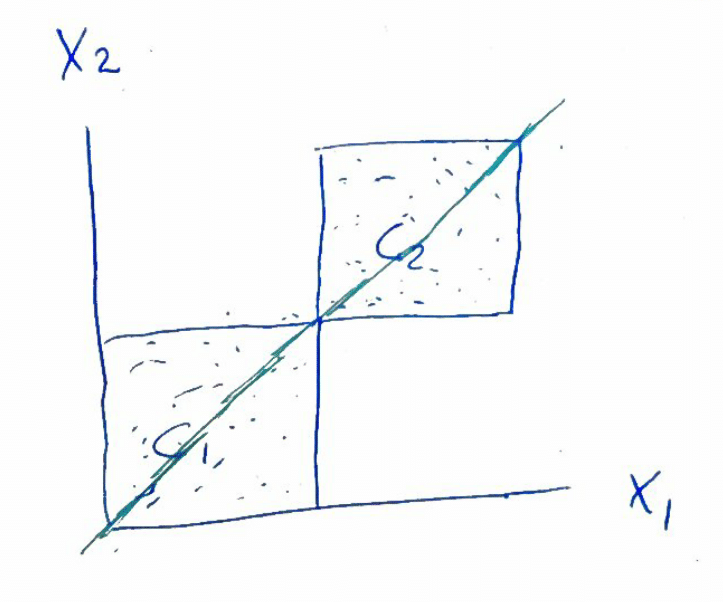
\includegraphics[width=0.7\textwidth]{tema_5/images/tema_5-6}
	\begin{tikzpicture}
		\begin{axis}[
				width=0.8\textwidth, height=0.7\textwidth,
				xmin = 0, xmax = 1.1,
				ymin = 0, ymax = 1.1,
				legend pos = north west,
				xlabel = $X_1$, ylabel = $X_2$,
				axis y line = left,
				axis x line = bottom,
				yticklabels = {,,},
				xticklabels = {,,},
			]
			\addplot+[only marks] table[x=x, y=y] {tema_5/data/bayes-1.csv};
			\addplot+[only marks] table[x=x, y=y] {tema_5/data/bayes-2.csv};
			\addplot+[mark=none]{x};
			\legend{$C_1$, $C_2$};
		\end{axis}
	\end{tikzpicture}
\end{figure}

$X_1$ i $X_2$ semblen dependents a primera vista però si només ens centrem en un dels dos conjunts llavors deixen de ser-ho.

\documentclass[a4paper]{article}
%\usepackage[margin=2cm]{geometry}

\usepackage{amsmath}
\usepackage{amssymb}
\usepackage{amsfonts}
\usepackage{mathtools}
\usepackage[catalan]{babel} % Language 
\usepackage{fontspec}
\usepackage{graphicx}
\usepackage[makeroom]{cancel}
\usepackage{float}
\usepackage{enumerate}
\usepackage{pgfplots}
\usepackage[hidelinks]{hyperref}
\usepackage{listings}

\pgfplotsset{compat=1.13}

\setlength{\parindent}{0pt}
\setlength{\parskip}{0.2cm}

\title{Tema 6: Classificadors probabilístics discriminatoris}
\author{Joan Marcè Igual}

\begin{document}
\maketitle
\section{Introducció}
Ja s'havia vist anteriorment que \textbf{LDA}:

$$
P(C_k|X) = \frac{P(X|C_k)P(C_k)}{\sum_{j=1}^K P(X|C_j)P(C_j)}\quad k=1,...,K
$$
$$
g(z) = \frac{1}{1 + e^{-z}}
$$

\textbf{Nº de paràmetres:}

$$
\Sigma_{d\times d} =
\begin{pmatrix}
d & & TS \\
& \ddots & \\
TI & & d
\end{pmatrix} \quad TS = TI \qquad 
\boxed{n = \frac{d(d+1)}{2} + Kd \sim O(d^2)}
$$

El nombre de paràmetres creixen quadràticament. De manera que aquests tipus de mètodes només serveixen per conjunts amb moltes dades.

En els classificadors discriminatius no es modelarà la forma de les classes. Es parteix del model $P(C_1|X) = g(w^T X + w_0)$. La idea és optimitzar els $w \in \mathbb{R}^d,w_0 \in \mathbb{R}$ directament (sense assumir cap distribució de les dades condicionades a la classe). Quants paràmetres s'han d'estimar? Doncs $d + 1 \in O(d)$ 

Per simplificar,
$$
w = \begin{pmatrix}
w_0 \\
w_1 \\
\vdots\\
w_d
\end{pmatrix}
\qquad
x = 
\begin{pmatrix}
x_0 = 1\\
x_1\\
\vdots\\
x_d
\end{pmatrix}
$$

Construïm la \textbf{menys log-versemblança de la mostra}:
$$
\mathcal{D} = \{ (x_1,t_1), ..., (x_N,t_N) \} 
\quad x_n \in \mathbb{R}^d
\quad t_n \in \{0, 1\}
\quad
\begin{cases}
0 \text{ vol dir } C_2 \\
1 \text{ vol dir } C_1
\end{cases}
$$
$$
P(t|x,w) =
\begin{rcases}\begin{cases}
g(w^T x) &\text{ si } t = 1 (x \in C_1)\\
1 - g(w^T x) &\text{ si } t = 0 (x \in C_2)
\end{cases}
\end{rcases}
= g(w^T x)^t · [1 - g(w^T x)]^{1 - t}
$$
\begin{flalign*}
	& -l(w) = -\ln \mathcal{L}(w) = -\ln P(\mathcal{D}|w) = 
	-\ln \prod_{n=1}^N P(t_n| x_n, w) \underbrace{=}_{\text{modelem}} \\
	& 5-\ln \prod_{n=1}^N g(w^T x_n)^{t_n} · [1 - g(w^T x_n)]^{1 - t_n} = \\
	& \sum_{n=1}^N \{ t_n \ln g(w^T x_n) + (1 - t_n) \ln(1 - g(w^T x_n)) \} \underbrace{=}_{\text{Defineixo } y_n := g(w^T x_n)} \\
	& -\sum_{n=1}^N \{ t_n \ln y_n + (1 - t_n) \ln (1 - y_n) \}
\end{flalign*}
$$
g'(z) = g(z)[1 - g(z)] \implies \\
g'(w^T x_n) = g(w^T x_n)·[1 - g(w^T x_n)] = y_n (1 - y_n)
$$
\begin{flalign*}
&\textbullet -\sum_{n=1}^N \left\{ \frac{t_n}{y_n}·g'(w^T x_n)·x_n - \frac{1 - t_n}{1 - y_n}·g'(w^T x_n) \right\} =\\
& -\sum_{n=1}^N t_n(1 - y_n)x_n - (1 - t_n)y_n x_n = \\
&- \sum_{n=1}^N \{ t_nx_n - \cancel{t_n y_n x_n} - y_n x_n + \cancel{t_n y_n x_n} \} = \\
& - \sum_{n=1}^N (t_n x_n - y_n x_n) = -\sum_{n=1}^{N} (t_n - y_n) x_n =
\boxed{\sum_{n=1}^N (y_n - t_n)x_n }
\end{flalign*}

\section{El mètode de Newton-Raphsum (NR)}
Va molt bé quan la funció a optimitzar és convexa. Per minimitzar $E(w)$ convexa, es fa el pas següent:
$$
\boxed{w^{\text{(nou)}} := w^{\text{(vell)}} - H^{-1} (w^{\text{(vell)}}) · \nabla E(w^{\text{(vell)}})}
$$
$$
\nabla E(w) =
\begin{pmatrix}
\frac{\partial E}{\partial w_0} \\
\frac{\partial E}{\partial w_1} \\
\vdots\\
\frac{\partial E}{\partial w_d}
\end{pmatrix}
\qquad
H(w) = \left( \frac{\partial^2 E}{\partial w_i \partial w_j} \right)
$$

\begin{lstlisting}[escapeinside={(*}{*)},frame=single]
inicialitzem w(0)
	i := 0
repetir
	w(i + 1) := w(i) - (*$H^{-1}$*)(w(i))·(*$\nabla$*)E(w(i))
	i = i + 1
fins que convergeix
\end{lstlisting}

\subsection{Aplicació af = E(w)}

$$
\nabla E = \sum_{n=1}^N (y_n - t_n) x_n = X^T(y-t)
$$
$$
X_{N\times (d+1)} =
\begin{pmatrix}
\longleftarrow x_1 \longrightarrow \\
\longleftarrow x_2 \longrightarrow \\
\vdots
\longleftarrow x_N \longrightarrow
\end{pmatrix}
\qquad
H = X^T R X
$$
$$
R := diag(y_1(1 - y_1), ..., y_N(1 - y_N))
$$


\subsection{L'algoritme IRLS}
\begin{lstlisting}[escapeinside={(*}{*)},frame=single]
inicialitzar: 
	w(0)(*$_0$*) := (*$\ln \frac{P(C_1)}{P(C_2)}$*)
	w(0)(*$_{1...d}$*) := 0
	i := 0
repetir
	(*$y_n := g(w^T(i)x_n),\ n=1,...,N$*)
	R := diag((*$y_1(1 - y_1),...,y_N(1 - y_N)$*))
	z := (*Xw(i) - $R^{-1}$*)(y - t)
	w(i + 1) := (*$(X^T R X)^{-1} X^T R z$*)
	i := i + 1
fins que convergeix
	(*$R^{-1} = \left( \frac{1}{y_1(1 - y_1)},..., \frac{1}{y_N(1 - y_N)} \right)$*)

Deviance
	D := -2*E(w)
	
Null deviance
	ND := -2*E(w(0))
\end{lstlisting}

\textbf{AIC} D + 2d
Regressió Logística $\rightarrow$ \texttt{RegLog}

\section{Interpretació de \texttt{RegLog}(I)}
$$
y(x, w) = g(w^T x) = P(C_1|x)
$$
$$
g(z) = \frac{1}{1 + e^{-z}} \qquad g^{-1}(z) =  \ln\left(\frac{z}{1 - z}\right)
$$
$$
w^T x = g^{-1} (P|C_1|x) = \ln\left( \frac{P(C_1|x)}{1 - P(C_1|x)} \right)
$$

\section{Interpretació de \texttt{RegLog}(III)}
Fixem un punt $x^* \in \mathbb{R}^d$ que volem predir (w és el vector solució).
$$
\frac{P(C_1|x^*)}{P(C_2|x^*)} = \exp(w^T x^*)
\qquad 1_i := (\underbrace{0,0,...}_{i - 1},1,...,0)^T
$$
$$
\frac{\frac{P(C_1|x^* + 1_i)}{P(C_2|x^* + 1_i)}}{\frac{P(C_1|x^*)}{P(C_2|x^*)}} =
\exp(w^T(\cancel{x^*} + 1_i) - \cancel{w^T x^*}) = 
\exp(w^T 1_i) = \exp(w_i)
$$

\end{document}
\chapter{Xarxes neuronals (artificials)}
\section{Introducció}
Models $y(x) = g(w^T \phi (x)),\ x \in \mathbb{R}^d, w \in \mathbb{R}^{d + 1}$.
$$
\phi(x) = 
\begin{pmatrix}
\phi_0(x) = 1 \\
\phi_1(x)\\
\vdots\\
\phi_M(x)
\end{pmatrix}
\quad 
g : f_n \ g:\mathbb{R} \rightarrow \mathbb{R} \text{(inversa global)}; 
\quad \phi : \mathbb{R}^d \rightarrow \mathbb{R}^M
$$
$$
X_{N \times d+ 1} \xrightarrow{\phi} \Phi_{N \times (M + 1)}
$$

La manera usual d'obtenir models \emph{no lineals} és establir funcions de base \emph{parametritzades}. La presència d'aquests paràmetres no lineals fa que les $\phi$ no es puguin pre-calcular.

En Xarxes Neuronals, la tria d'aquestes funcions de base es fa de la següent manera:
$$
\phi_i(x) := \phi (\psi(x, v_i))
$$
\begin{align*}
	&v_i & \text{és un vector de paràmetres (no lineals)} \\
	&\psi : \mathbb{R}^d \times \mathbb{R}^d \rightarrow \mathbb{R}
	& \text{és una funció de combinació} \\
	&\phi : \mathbb{R} \rightarrow (a,b) &
	\text{és una funció d'activació}
\end{align*}

$\psi$ calcula una similitud entre dos vectors: $x_1 v_i$.
$\phi$ determina el valor final d'activació de $\phi_i$.

\textbf{Definició}: diem que una funció $\phi \mathbb{R} \rightarrow (a,b)$ és \emph{sigmoidal} si:
\begin{enumerate}
	\item $\lim\limits_{z \rightarrow - \infty} \phi(b) = a$
	\item $\lim\limits_{z \rightarrow + \infty} \phi(z) = b$
	\item $\phi'(z) > 0,\ \forall z \qquad \phi'(z) < 0,\ \forall z$ i $\phi'$ té forma de campana.
\end{enumerate}

\textbf{Exemples}:

\begin{enumerate}
	\item La funció logística $\phi(z) = \frac{1}{1 + e^{-z}} \in (0, 1)$
	\begin{figure}[H]
		\centering
		\begin{tikzpicture}
		\begin{axis}[
		xmin=-7,xmax=7,ymin=0,ymax=1,
		domain=-10:10,
		axis x line=center,
		axis y line=center
		]
		\addplot+[mark=none] {1/(1 + exp(-x))};
		\end{axis}
		\end{tikzpicture}
		\caption{Gràfic funció logística}
		\label{fig:logistic}
	\end{figure}

	\item La tangent hiperbòlica $\phi(z) = \frac{e^z - e^{-z}}{e^z + e^{-z}} \in (0,1)$.
	
	\begin{figure}[H]
		\centering
		\begin{tikzpicture}
		\begin{axis}[
		xmin=-5,xmax=5,ymin=-1.05,ymax=1.05,
		domain=-5:5,
		axis x line=center,
		axis y line=center
		]
		\addplot+[mark=none] {(exp(x) - exp(-x))/(exp(x) + exp(-x))};
		\end{axis}
		\end{tikzpicture}
		\caption{Gràfic funció inversa hiperbòlica}
		\label{fig:inv_hiperbol}
	\end{figure}
\end{enumerate}

$$
\implies y(x) = g(w^T \phi(x)) = g\left(\sum_{i=0}^M w_i \phi_i(x)\right) = g \left( \sum_{i=0}^M w_i \phi(v_i^T x + v_{i0}) \right)
$$
\begin{itemize}
	\item $w_i$ són paràmetres lineals
	\item $v_i$ i $v_{i0}$ són paràmetres no lineals
\end{itemize}

% FIGURA 1

Si es dediquen esforços a optimitzar una funció que té molts mínims locals es pot arribar a un mínim que no sigui un mínim absolut. Això dificulta molt la feina d'optimització. Tot i així l'error al que s'acaba arribant al final resulta ser només un error amb les dades d'entrenament. 

Per tant, amb les dades més genèriques l'error també serà menor. Si es minimitzessin al màxim les dades d'entrenament llavors amb les altres potser no s'aconsegueix un mínim.

% FIGURA 2

A cada $ \phi_i(x) $ se li diu \emph{neurona}.

\begin{figure}[H]
	\centering
	\begin{tikzpicture}[x=1.5cm, y=1.5cm, >=stealth]
	
	
	\node (input) at (0,0) {$
		\begin{pmatrix}
		I_1 \\ I_2 \\ \vdots \\ I_N
		\end{pmatrix}
		$};
		
	\foreach \m [count=\y] in {1,missing,2}
	\node [every neuron/.try, neuron \m/.try ] (hidden-\m) at (2,2-\y*1.25) {\ifthenelse{\equal{\m}{missing}}{}{$S(\Sigma)$}};
	
	\foreach \m [count=\y] in {1,missing,2}
	\node [every neuron/.try, neuron \m/.try ] (output-\m) at (4,1.5-\y) {\ifthenelse{\equal{\m}{missing}}{}{$g(\Sigma)$}};
	
	\foreach \l [count=\i] in {1,M}
	\node [above] at (hidden-\i.north) {$\phi_\l$};
	
	\foreach \l [count=\i] in {1,n}
	\draw [->] (output-\i) -- ++(1,0)
	node [above, midway] {$O_\l$};
	
	\foreach \i in {1,...,2}
	\draw [->] (input) -- (hidden-\i);
	
	\foreach \i in {1,...,2}
	\foreach \j in {1,...,2}
	\draw [->] (hidden-\i) -- (output-\j) node [midway,above,sloped] {$w_{\i\j}$};
	
	\foreach \l [count=\x from 0] in {Input (abstract), Hidden, Ouput}
	\node [align=center, above] at (\x*2,2) {\l \\ layer};
	
	\end{tikzpicture}
\end{figure}

\begin{itemize}
	\item La xarxa treballa "endavant" quan ho fa en el sentit de les fletxes $\rightarrow$.
	\item La capa de \emph{sortida} és la darrera capa endavant
	\item Les capes \emph{ocultes} són totes excepte la de sortida (les seves \emph{neurones} també es diuen \emph{ocultes}).
	\item No hi ha capa "d'entrada".
\end{itemize}

A vegades tenim múltiples capes ocultes

\begin{figure}[H]
	\centering
	\begin{tikzpicture}[x=1.5cm, y=1.5cm, >=stealth]
		\node (input) at (0,0) {$
			\begin{pmatrix}
			I_1 \\ I_2 \\ \vdots \\ I_N
			\end{pmatrix}$};
		
		\foreach \m [count=\y] in {1,2,missing,3} 
		\node [every neuron/.try, neuron \m/.try](hidden-1-\m) at (2,2.5 - \y*1.25){};
		
		\foreach \m [count=\y] in {1,2,missing,3} 
		\node [every neuron/.try, neuron \m/.try](hidden-2-\m) at (4,2.5 - \y*1.25){};
		
		\node [every neuron/.try](output) at(6,0){};
		
		\foreach \i in {1,...,3}
		{
			\draw[->](input) -- (hidden-1-\i); 
			\draw[->](hidden-2-\i) -- (output); 
			\foreach \j in {1,...,3}
			{ 	
				\draw[->](hidden-1-\i) -- (hidden-2-\j);
			}
		}
	
		\foreach \l [count=\x from 0] in {Input (abstract), Hidden 1, Hidden 2, Ouput}
		\node [align=center, above] at (\x*2,2) {\l \\ layer};
	\end{tikzpicture}
\end{figure}

$$
y(x) = g\left(\sum_i w_i\phi_i(x)\right) =
g\left(\sum_i w_i \phi (v_i^T x) \right) =
g\left( \sum_i w_i \phi \left(\sum_j v_{ij} x_j\right)  \right)
$$
En aquest cas $x_j \rightarrow \gamma_i (x) = \phi (z_j^T x + z_{j0})$. Per tant:
$$
y(x) = g\left( \sum_i w_i \phi \left( \sum_j w_{ij} \phi \left( z_{jn} x_n + x_{n0} \right) + v_{j0} \right) + w_0 \right)
$$

\subsection{La funció g}

\begin{table}[H]
	\centering
	\setlength\extrarowheight{15pt}
	\begin{tabular}{p{2.2cm}|p{2.3cm}p{3cm}p{2.8cm}}
		& Regressió & \parbox{2cm}{Classificació \\ ($K=2$)} & \parbox{2cm}{Classificació \\ ($K > 2$)} \\
		\hline
		Funció g & g = Identitat & logística & softmax \\
		Funció d'error & error quadràtic & entropia creuada & entropia creuada generalitzada \\
		Interpretació de la sortida & el target K-èsim (m neurones de sortida) & \parbox{3cm}{$y(x) = P(w_1 |X)$ \\ $\implies$ \\ $P(w_2|X) = 1 - g(x)$} (una neurona de sortida) &  \parbox{2.8cm}{$y_k(x) = P(w_k|X)$ \\ (K neurones de sortida)}
	\end{tabular}
\end{table}

\section{Entrenament de xarxes neuronals (Xarxes MLD)}
$$
y_{MLD}(x) = 
\begin{pmatrix}
y_1(x) \\
y_2(x) \\
\vdots \\
y_m(x)
\end{pmatrix},
\  x \in \mathbb{R}^d 
\quad y_{MLD}: \mathbb{R}^d \rightarrow \mathbb{R}^m
$$

\begin{itemize}
	\item Es tenen $c$ capes ocultes i 1 capa de sortida = $c + 1$ capes.
	\item $w_l$ és el nombre de neurones de la capa $l$
\end{itemize}

\begin{figure}[H]
	\centering
	\begin{tikzpicture}[x=1.5cm, y=1.5cm]
		\node[every neuron/.try] (i) at (0,0) {i};
		\node[every neuron/.try] (j) at (2,0) {j};
		\node[below = 0.3cm of i] {$(l - 1)$};
		\node[below = 0.3cm of j] {$(l)$};
		\draw[->] (i) to[bend left = 20] node[midway,above] {$w_{ji}^l$} (j);
	\end{tikzpicture}
\end{figure}
\begin{itemize}
	\item $\boldsymbol{w_l} = \begin{pmatrix}
	w_{ji}^l
	\end{pmatrix}_{j,i} \rightarrow$ vector $\forall$ parella $j,i$.
	\item $W = (w_l)_{l=1,...,c}$.
\end{itemize}


Es defineix:
\begin{align*}
	& z_j^l := \phi(a_j^l) \\
	& a_j^l := \sum_{i=0}^{h_{l-1}} w_{ji}^l z_i^{l-1}
\end{align*}

Es fixa l'exemple $n$. El primer que es fa és calcular les sortides de totes les neurones de la xarxa. Primer es calculen totes les $\delta_k$ de totes les $c$ capes ocultes.

\begin{align*}
	& \delta_k^{c+1} = t_{nk} - z_{k}^{c+1} \\
	& \delta_j^{l+1} \propto \sum_{k} w_{kj}^{l+1} · \delta_{k}^{c+1} \\
	& \Delta w_{kj}^{l+1} \propto \delta_k^{c+1} z_j^{l+1}	
\end{align*}

\begin{figure}[H]
	\centering
	\begin{tikzpicture}[x=1.5cm, y=1.5cm, >=stealth]
		\foreach \m [count=\y] in {1,2,missing,3}
		\node[every neuron/.try, neuron \m/.try](hidden-0-\m) at (0,2.5 - \y*1.25){};
		
		\foreach \m in {1,...,4}
		\node(intermid-\m) at (1,2.5 - \m*1.25){$\cdots$};
		
		\foreach \m [count=\y] in {1,2,missing,3}
		\node[every neuron/.try, neuron \m/.try](hidden-1-\m) at (2,2.5 - \y*1.25)
		{\ifthenelse{\equal{\m}{missing}}{}{$i$}};
		
		\foreach \m [count=\y] in {1,2,missing,3}
		\node[every neuron/.try, neuron \m/.try](hidden-2-\m) at (4,2.5 - \y*1.25)
		{\ifthenelse{\equal{\m}{missing}}{}{$j$}};
		
		\foreach \m [count=\y] in {1,2,missing,3}
		\node[every neuron/.try, neuron \m/.try](hidden-3-\m) at (6,2.5 - \y*1.25)
		{\ifthenelse{\equal{\m}{missing}}{}{$k$}};
		
		\foreach \m [count=\y] in {l, l+1, c+1}
		\node at (2*\y, -3){\m};
		
		\draw[->](hidden-1-1) to[out=30, in=150] node [sloped,midway,above]{$w_{ij}^{l+1}$} (hidden-2-1) ;
	\end{tikzpicture}
\end{figure}

\subsection{Algorisme \texttt{backprop}}

\texttt{backprop(D, "especificació de l'arquitectura")}

\begin{algorithmic}
	\State inicialitzar els pesos  $\forall j,l,i$
	\Repeat
	\For{$n := 1$ fins $N$} 
		\Comment{PAS FORWARD (sentit de les fletxes)}
		\State Calcular les sortides $z_j^l,\ \forall j,l$
		\Comment{PAS BACKWARD}
		\For{$l := c$ fins $1$}
			\If{$l = c$} 
				$\delta_j := (t_{nj} - z_{j}^{c+1})$
			\Else
				$\ \delta_j^l := \phi' (a_j^l) \sum_q w_{qj}^{l+1} z_j^l$
			\EndIf
		\EndFor
	\EndFor
	\ForAll{j,l,i}
		\State $\Delta w_{ji}^l := \sum_{n=1}^N \Delta w_{ji}^l$
		\State $w_{ji}^l := w_{ji}^l - \alpha \Delta w_{ji}^l$
	\EndFor
	\Until{Convergeixi}
\end{algorithmic}

\section{Xarxes de neurones de Base Radial}
RBF (\textsc{Radial Basis Function})

\begin{align*}
& \phi_i (x) = \phi\left( \frac{||x - m_i||}{h_i} \right)
\begin{cases}
h_i > 0: &\text{ paràmetre de suavització} \\
m_i: &\text{centre de la neurona } i
\end{cases} \\
& \phi:\mathbb{R}_0^+ \rightarrow \mathbb{R} \\
& \phi(z) = \exp\left( - \frac{z^2}{2} \right)
\end{align*}

\begin{figure}[H]
	\centering
	\begin{tikzpicture}
		\begin{axis}[
		xmin=-0,xmax=5,ymin=0,ymax=1.05,
		domain=0:5,
		samples=100,
		axis x line=center,
		axis y line=center
		]
		\addplot+[mark=none] {exp(-x^2/2))};			
		\end{axis}
	\end{tikzpicture}
\end{figure}
\subsection{Entrenament d'una xarxa RBF}
\subsubsection{Posicionar les neurones a l'espai d'entrada}
Usant un algorisme de \emph{clustering} (per exemple \texttt{k-means}), amb un nombre de clusters (M). Uaser el resultat del clustering per determinar:
\begin{itemize}
	\item Centre des les M neurones: centroides del clustering ($m_i$)
	\item Paràmetres de suavització ($h_i$).
	\begin{align*}
		& h_i \propto \frac{d_{\max}}{\sqrt{2M}} \qquad d_{\max}\ \text{entre centres (ct.)} \\
		& h_i \propto d_{mitjana} \ \text{entre centres (ct.)} \\
		& h_i \propto d_{mitjana} \ \text{entre el $m_i$ i les dades $x_n$ (diferent per cada i)}
	\end{align*}
\end{itemize}

\subsubsection{Tenim les funcions $\phi_i (x) = \phi\left( \frac{||x - m_i||}{h_i} \right)$}
\begin{itemize}
	\item Calculem la matriu de disseny $\Phi_{ij} = \phi_j(x_i)$.
\end{itemize}
\subsubsection{Regressió en $\Phi$}
\begin{itemize}
	\item regressió: regressió lineal regularitzada (ridge regression)
	\item classificació ($k=$ 2 classes): regressió logística
	\item classificació ($k>$ 2 classes): regressió multilineal
\end{itemize}

$$
y_{RBF}(x) = \sum_{i=1}^{M} w_i \phi_i(x) + w_0 \quad \text{(regressió lineal)}
$$

\subsection{Influència de $M$ i $\{h_i\}$}
\begin{itemize}
	\item $M$ neurones $\rightarrow$ sobreajust (a menys que hi hagi regularització)
	\item $h_i$?
\end{itemize}

$$
\phi_i(x) = \exp\left( - \frac{||x - m_i||^2}{h_i^2} \right)
$$

% FIGURA 1
Imaginem que tenim una funció i una sèrie de dades i es fa un clustering d'aquestes dades. Es posen unes quantes neurones i cadascuna d'aquestes té una resposta Gaussiana. 

El paràmetre de suavització fa que les Gaussianes siguin més estretes o més amples. Si es tria una $h_i = h$ per totes les neurones i llavors es fa que $h \rightarrow \infty$ llavors la resposta de totes les neurones serà molt plana i la resposta de la xarxa serà l'infra-ajust.

Per contra si la $h \rightarrow 0$ la resposta de les neurones serà molt local i la xarxa tendirà al sobre-ajust.

\documentclass[a4paper]{article}

\usepackage{amsmath}
\usepackage{amssymb}
\usepackage{amsfonts}
\usepackage{mathtools}
\usepackage[catalan]{babel} % Language 
\usepackage{fontspec}
\usepackage[makeroom]{cancel}
\usepackage[dvipsnames]{xcolor}
\usepackage{tikz}
\usepackage{pgfplots}
\usepackage{float}

\newcommand*{\op}[1]{\operatorname{#1}}
\newcommand*{\bmath}[1]{\boldsymbol{#1}}

\setlength{\parindent}{0pt}
\setlength{\parskip}{0.2cm}

\title{Tema 8: Màquines de vectors suport (Introducció als mètodes kernel)}
\author{Joan Marcè i Igual}

\begin{document}
\section{Introducció}

Estem treballant amb models de la forma:
$$
y(x) = g(\boldsymbol{w}^T\boldsymbol{\phi}(x) + w_0),\ x \in \mathbb{R}^d, w \in \mathbb{R}^M, w_0 \in \mathbb{R}^d
$$
$$
\boldsymbol{\phi}(x) =
\begin{pmatrix}
\phi_1(x) \\
\phi_2(x) \\
\vdots \\
\phi_M(x)
\end{pmatrix}
$$

En xarxes neuronals es va dir que $\phi_i(x) = \phi(\varphi(x, v_i))$. 

Ara calculem un model lineal en l'espai de representació generat per les $\phi_i(x)$ (\textbf{feature space} = espai de característiques). El que fan els mètodes no lineals és buscar l'espai d'estadístiques adequat per a un problema en concret.

Una manera diferent de treballar és estudiar l'expressió:
\begin{align*}
	\phi(x)^T\phi(y) \quad x,y \in \mathbb{R}^d \\
	\phi: \text{feature map} 
\end{align*}

\textbf{Definim:} una funció de kernel $k: \mathbb{R}^d \times \mathbb{R}^d \rightarrow \mathbb{R}$ com:
$$
k(x,y) := \phi(x)^T\phi(y)
$$

\begin{itemize}
	\item Es poden estudiar les propietats de $k$ sense calcular (ni tan sols conèixer) $\phi$ de manera explícita.
	\item Es pot obtenir un algorisme d'aprenentatge \textbf{no lineal} partir d'un de lineal mitjançant l'ús de funcions de kernel (\emph{kernelitzar}).
	$$
	x^Ty \rightarrow \underbrace{\phi(x)^T\phi(y)}_{\mathclap{\text{$\phi$ no lineal, el resultat és un algorisme no lineal}}} = k(x,y)
	$$
\end{itemize}

\section{Com construir funcions de kernel}
Si tenim un 
$$
\phi(x) = 
\begin{pmatrix}
\phi_1(x)\\
\phi_2(x) \\
\vdots \\
\phi_n(x)
\end{pmatrix}
$$
$$
\implies k(x,y) = \phi^T(x)\phi(x) = \sum_{i=1}^M \phi_i(x)\phi_i(y)
$$

\textbf{Exemple} $(x^Ty)^3 \ ,x,y \in \mathbb{R}^3$
$$
x = \begin{pmatrix}
x_1 \\
x_2 \\
x_3
\end{pmatrix};
\quad 
y = \begin{pmatrix}
y_1 \\
y_2 \\
y_3
\end{pmatrix}
$$
\begin{align*}
	& (x^Ty)^3 = (x_1y_y + x_2y_2 + x_3y_3) = \\
	& (x_1y_1)^3 + 3(x_1y_1 + x_2y_2)^2 x_3y_3 + 3(x_1y_1 +
	 x_2y_2)(x_3y_3)^2 + (x_3y_3)^3 = ... \\
	& = 
	\begin{pmatrix}
	x_1^3 \\
	x_2^3 \\
	x_3^3 \\
	\sqrt{6} x_1x_2x_3 \\
	\sqrt{3} x_1^2x_2 \\
	\sqrt{3} x_1^2x_3 \\
	\sqrt{3} x_2^2x_1 \\
	\sqrt{3} x_2^2x_3 \\
	\sqrt{3} x_3^3x_1 \\
	\sqrt{3} x_3^3x_2 \\
	\end{pmatrix}^T 
	\begin{pmatrix}
	y_1^3 \\
	y_2^3 \\
	y_3^3 \\
	\sqrt{6} y_1y_2y_3 \\
	\sqrt{3} y_1^2y_2 \\
	\sqrt{3} y_1^2y_3 \\
	\sqrt{3} y_2^2y_1 \\
	\sqrt{3} y_2^2y_3 \\
	\sqrt{3} y_3^2y_1 \\
	\sqrt{3} y_3^2y_2
	\end{pmatrix}
	= \phi(x)^T\phi(y) \qquad \phi:\mathbb{R}^3 \rightarrow \mathbb{R}^{10}
\end{align*}

% FIGURA 2

$$
(x^Ty + 1)^3 \implies
$$
$\phi$ calcula tots els monomis de les variables (1,...,d) fins a grau 3. (0, 1, 2, 3).

$x^Ty$ \textbf{kernel lineal}

$\phi(x) = x$

$(x^Ty + 1)^2$ kernel quadràtic

$(x^Ty + 1)^3$ kernel cúbic

$(x^Ty + c)^q \quad ,c \ge 0, q \in \mathbb{N}$ kernel polinòmic

\textbf{Teorema} Una funció $k:\mathbb{R}^d \times \mathbb{R}^d \rightarrow \mathbb{R}$ és una \textbf{funció lineal} ($\exists \phi: \mathbb{R}^d \rightarrow \mathbb{R}^D, t.q. \ k(x,y) = \phi^T(x)\phi(y)$) si i només si:
\begin{itemize}
	\item $k$ és simètrica
	$$
		k(x,y) = k(y,x) \quad ,\forall x,y \in \mathbb{R}^d
	$$
	\item $\forall N \in \mathbb{N}$, per tota tria $x_1,...,x_N \ \mathbb{R}^d$, la matriu $K_{i,j} := k(x_i, x_j)$ és semi-definida positiva (PSD)
\end{itemize}

\textbf{Definició:} diem que una matriu $K_{N \times N}$ és PSD si és simètrica i $\forall c \in \mathbb{R}^N, c^T K c \ge 0$. És a dir $\sum_{i=1}^N\sum_{j=1}^N c_i K_{ij} c_j \ge 0$.

\textbf{Demostració:} Si la funció $k$ és un kernel $\implies K$ és PSD.
\begin{align*}
	& \sum_i \sum_j c_i K_{ij} c_j = 
	\sum_i \sum_j c_i \phi^T(x_i) \phi(x_j)c_j = \\
	& \left( \sum_i c_i \phi(x_i) \right)^T
	\left( \sum_j c_j \phi(x_j) \right) = 
	\left|\left| \sum_i c_i \phi(x_i) \right|\right|^2 \ge 0
\end{align*}

\textbf{Propietats}
Si $k$, kernels, $a \in \mathbb{R} \quad a \ge 0$:
\begin{itemize}
	\item $a·k$ kernel
	\item $k_1 + k_2$ kernel
	\item $k_1·k_2$ kernel
	\item p(k) kernel, si p és un polinomi de coeficients no negatius
\end{itemize}

\textbf{Proposició}
$$
k(x,y) = (x^Ty + c)^q \quad \forall c \ge 0, \forall q \in \mathbb{N}
$$

Podem definir funcions de kernel en qualsevol conjunt d'objectes o espai.
$$
k: \mathbb{R}^d \rightarrow \mathbb{R}^d 
\rightarrow \mathbb{R} \implies 
k: X \times X \rightarrow \mathbb{R}
$$
$X$ conjunt d'objectes finit (persones).

Una manera de comparar dos conjunts és comparar quants elements tenen en comú
$$
k(x,y) = | x \cap y|
$$
$$
x,y \subset X
$$
$$
I_X (M) = \begin{cases}
1 & \text{ si } M \in X \\
0 & \text{ si } M \cancel{\in} X
\end{cases}
$$
$$
|x \cap y| = \sum_{u \in X} I_X(u)·I_y(u) = k(x,y)
$$

\section{La dimensió VC per classificadors}
Es mesura la complexitat d'un model, per a un model lineal aquesta depèn del nombre de paràmetres. 

Sigui $\mathcal{F} = \{ y : \mathbb{R}^d \to \{ -1, +1 \} : y_0 \text{ està parametritzat per } \theta \in H \}$. Es fixen unes dades $\mathcal{D} = \{ (x_1, t_1),..., (x_N, t_N) \}$. Es diu que un classificador $y_0 \in \mathcal{F}$ trenca/esmicola (scatter) $\mathcal{D}$ si, per tota tria de les $t_n \ (1 \le n \le N)$ (hi ha $2^n$ tries diferents) $y_0$  classifica correctament les $x_n$.

\textbf{Definició} 

La dimensió VC de $\mathcal{F}$ és la $N$ més gran per la qual existeixen $x_1, ..., x_N \in \mathbb{R}$  tals que $\exists y_0 \in \mathcal{F}$ que les trenca (per a qualsevol configuració). 

\textbf{Exemple}

$$
\mathcal{F}_{lin}^d = \{ y(\boldsymbol{x}, \boldsymbol{w}) = signe(\boldsymbol{w}^T \boldsymbol{x} + w_0), 
\ \boldsymbol{x} \in \mathbb{R}^d, \ \boldsymbol{w} \in \mathbb{R}^d, \ w \in \mathbb{R}  \}
$$

\textbf{Proposició}: $\dim (\mathcal{F}_{lin}^d) = d + 1$.

\section{Màquines de Vectors Suport}

\begin{figure}[H]
	\centering
		
	\begin{tikzpicture}[scale=8]
		\draw [step=0.1, dotted, gray] (-0.5,0) grid (0.5,0.6);
	
		\foreach \Point [count=\x] in {(0.09, 0.25), (0.25, 0.05), (0.4, 0.3), (0.25, 0.5), (0.11, 0.55), (0.2, 0.3), (0.25, 0.4)}{
			\node (right-\x) at \Point {\textbullet};
		}
		\foreach \Point [count=\x] in {(-0.15, 0.1), (-0.3, 0.09), (-0.4, 0.35), (-0.25, 0.59), (-0.12, 0.45), (-0.2, 0.27), (-0.25, 0.33)} {
			\node (left-\x) at \Point {$\circ$};
		}
	
		\foreach \x [remember=\x as \lastx (initially 1)] in{2,...,5,1}{
			\draw (right-\x) -- (right-\lastx);
			\draw (left-\x) -- (left-\lastx);
		}
	
		\draw[very thick, Green] (0,0) -- (0, 0.6) node[at start, right] {\textcolor{Green}{$m = $ marge}};
		
		\node[text width = 4cm] at (0.6, 0.6) {Polígon convex de superfície interior mínima que abarca tots els punts de la classe};
	\end{tikzpicture}
\end{figure}

Si es suposa que les dades són separables linealment. Es busca la recta que les separa deixant un marge $m$ màxim.

\begin{align*}
	\mathcal{D} &= \{ (x_1, t_1), ..., (x_N, t_N) \} \quad \text{S'assumeix $\mathcal{D}$ és separable linealment} \\
	& \phantom{{}={}}  
	\begin{aligned}
		\text{\textbf{def }} & y(x) = \op{sgn}(\boldsymbol{w}^T \boldsymbol{x} + w_0) \\
		& \text{on } \op{sgn}(z) = 
		\begin{cases}
			1 & \text{ si } z > 0 \\
			-1 & \text{ si } z < 0
		\end{cases}
	\end{aligned}
\end{align*}

\begin{align*}
	& \left[ \forall n : 1 \le n \le N : 
	\begin{rcases}
	\begin{cases}
		\bmath{w}^T x_n + w_0 > 0 & \text{ si } t_n = +1 \\
		\bmath{w}^T x_n + w_0 < 0 & \text{ si } t_n = -1
	\end{cases}
	\end{rcases} 
	\right] \\
	& \hspace{2em} \Updownarrow \\
	& \left[ \forall n : 1 \le n \le N : (\bmath{w}^T x_n + w_0) t_n > 0 \right]
\end{align*}

\textbf{Definició}: El \textbf{marge} d'un pla $\pi := $ distància de $\pi$ al punt més proper.

\textbf{Definició}: El \textbf{pla separador òptim} (PSO) $:=$ pla $\pi$ de màxim marge.

$$
\pi \left| \max_{\bmath{w}, w_0} \left( \min_{1 \le n \le N} d(x_n, \pi) \right)\right.
$$

Es normalitza $\bmath{w} \scalebox{1.8}{|} |\bmath{w}^T \bmath{x} + w_0| \ge 1$:

\textbf{Definició}: Els punts $x_n \scalebox{1.8}{|} |\bmath{w}^T \bmath{x} + w_0| = 1$ es diuen \textbf{vectors suport} (VS). 

\begin{itemize}
	\item El marge del PSO $\pi$ és: $d(x_{vs}, \pi) = 2 \frac{|\bmath{w}^T \bmath{x}_{vs} + w_0}{||w||} = \frac{2}{||w||}$
\end{itemize}

Així doncs el problema a resoldre s'escriu:

$$
\boxed{
\begin{aligned}
& \min_{\bmath{w},w_0} \frac{||w||^2}{2} \quad \text{Maximitzar el marge} \\
& \text{\textbf{subjecte a }} t_n (\bmath{w}^T x_n + w_0) \ge 1, \quad \forall n : 1 \ge n \ge N
\end{aligned}
}
$$

\textbf{Teorema} (Vapnik)

Es considera una classe de models $\mathcal{F}$ amb $\op{dimVC}(\mathcal{F}) = h$, amb probabilitat de com a mínim $1 - \eta$ on:

\begin{itemize}
	\item $E(y_D) \le E_D (y_D) + H(h, \eta, N)$ 
	\item $E(y_D)$ és l'error de generalització de $y_D$
	\item $E_D(y_D)$ és l'error de training de $y_D$ en les dades $\mathcal{D}$
	\item $y_D$ és un model de $\mathcal{F}$ obtingut amb les dades $\mathbb{D}$
	\item $H(h, \eta, N) = \left( \frac{h(\ln \frac{2N}{\eta} + 1) - \ln \frac{y}{4}}{N} \right)^{\frac{1}{2}}$ complexitat
\end{itemize}

\textbf{Teorema}

Sigui $\mathcal{F} = \{ y(x) = \op{sgn}(w^T x + w_0), \ w \in \mathbb{R}^d, \ w_0 \in \mathbb{R} \}$, considerem la subclasse $\mathcal{F}_n \subset \mathcal{F}$ que té marge $m \implies \dim VC(\mathcal{F}_m) \le \min \left( \left\lceil \frac{R^2}{m^2} \right\rceil, d \right) + 1$. On $R$ és el radi de l'esfera més petita que conté les dades. 

\subsection{Violacions del marge}

% Copiar d'Arnau, full 8-4

\begin{figure}[H]
	\centering
	\begin{tikzpicture}
		\begin{axis}[
				xmin=-0.1, xmax=1.1,
				ymin=-0.1, ymax=1.1,
				width=0.9\textwidth,
				height=0.9\textwidth
			]
			\addplot[blue, only marks] table [x=x, y=y]{data/data1.csv};
			\addplot[red, only marks] table [x=x, y=y]{data/data2.csv};
			\addplot[green, mark=none, very thick] {0.5};
			\addplot[green, mark=none] {0.55};
			\addplot[green, mark=none] {0.45};
			\addplot[purple, mark=none, very thick]{-x + 1};
			\addplot[purple, mark=none]{-x + 1.2};
			\addplot[purple, mark=none]{-x + 0.8};
			\draw[->] (axis cs:0.5,0.5) -- (axis cs:0.6,0.6) node[sloped, midway, above] {$m_2$};
			\draw[->] (axis cs:0.5,0.5) -- (axis cs:0.4,0.4) node[sloped, midway, above] {$m_2$};
			\draw[->] (axis cs:0, 0.5) -- (axis cs: 0, 0.55) node[midway, right] {$m_1$};
			\draw[->] (axis cs:0, 0.5) -- (axis cs: 0, 0.45) node[midway, right] {$m_1$};
			\draw[->] (axis cs:1, 0.5) -- (axis cs: 1, 0.55) node[midway, left] {$m_1$};
			\draw[->] (axis cs:1, 0.5) -- (axis cs: 1, 0.45) node[midway, left] {$m_1$};
		\end{axis}
	\end{tikzpicture}
\end{figure}


Si en lloc de separar les dades perfectament es tria un altre separador que cometi un cert error es pot aconseguir disminuir la dimensió VC del classificador. D'aquesta manera es pot violar el marge de separació per tal de disminuir la dimensió VC del classificador. \emph{Com s'escull aquesta violació? Quin nou marge s'escull? Com es quantifica la violació de marge?} El control del marge permet controlar el sobre-ajust també. 

\begin{itemize}
	\item Un cop es permeten aquestes violacions hi ha un compromís entre \emph{l'ajust de les dades} (separar tots els punts tant com sigui possible) i reduir \emph{la complexitat} (maximitzar el marge).
	
	\item S'introdueix un paràmetre de ponderació (\emph{cost parameter}): $C > 0$.
	
	$$
	\frac{min}{w_1 w_0 \textcolor{red}{,\varepsilon}} \frac{1}{2} ||w||^2 \textcolor{red}{+} \textcolor{Green}{C} \textcolor{red}{\cdot \sum_{n=1}^N \varepsilon_n}
	$$
	
	Subjecte a $t_n (w^T x_n + w_0) \ge 1; \quad (1 \le n \le N); \quad \textcolor{red}{\varepsilon_n \ge 0}$
	
	\begin{align*}
		& \textcolor{Green}{C \to \infty} & \textcolor{Green}{m \downarrow} & 
		\textcolor{Green}{\text{ sobreajust}} & \textcolor{Green}{\text{(separador 1)}} &
		\textcolor{Green}{\text{ errors de training } \downarrow} \\
		& \textcolor{red}{C \to 0} & \textcolor{red}{m \uparrow} & 
		\textcolor{red}{\text{ infrajust}} & \textcolor{red}{\text{(separador 2)}} &
		\textcolor{red}{\text{ errors de training } \uparrow}
	\end{align*}
\end{itemize}

\begin{align*}
	\mathcal{L} =& \frac{1}{2} ||w||^2  + C \cdot \sum_{n=1}^N \varepsilon - 
	\underbrace{\sum_{n=1}^N \mu_n \varepsilon_n}_{
		\mathclap{\text{\parbox{2cm}{restriccions \\ $\varepsilon_n \ge 0$}}}} 
	-\underbrace{\sum_{n=1}^N \alpha_n \{ t_n (w^T x_n + w_0) - 1 + \varepsilon_n \}}_{\mathclap{
		\text{\parbox{4cm}{restriccions \\ 
				$t_n (\bmath{w}^T \bmath{x_n} + w_0) + \varepsilon_n + 1 \implies$ \\
				$-t_n (\bmath{w}^T \bmath{x_n} + w_0) - \varepsilon_n + 1 \le 0 $ }}
	}} 
	\\
	& \alpha_n \ge 0 \\
	& \mu_n \ge 0
\end{align*}

\begin{align*}
	& \textbullet \frac{\partial \mathcal{L}}{\partial w_0} = - \sum_{n=1}^N \alpha_n t_n = 0 \implies \boxed{\sum_{n=1}^N \alpha_n t_n = 0} \\
	& \textbullet \frac{\partial \mathcal{L}}{\partial w} = w - \sum_{n=1}^N \alpha_n t_n x_n = 0 \implies \boxed{w = \sum_{n=1}^N \alpha_n t_n x_n} \\
	& \textbullet \frac{\partial \mathcal{L}}{\partial \epsilon_n} = C - \alpha_n - \mu_n = 0  \implies \boxed{C= \alpha_n + \mu_n}
\end{align*}
	
Substituim en $\mathcal{L}$ i obtenim el lagrangià dual $\mathcal{L}_{dual}$:

$$
\boxed{
\begin{aligned}
	&\mathcal{L}_{dual} = \sum_{n=1}^N \alpha_n - 
	\frac{1}{2} \sum_{n=1}^N \sum_{m=1}^N \alpha_n \alpha_m t_n t_m \textcolor{red}{x_n^T x_m} \\
	&\text{Subjecte a } 0 \le \alpha_n \le C
\end{aligned}
}
$$

\textcolor{red}{Kernelització! Substituïm $x_n$ per $\phi (x_n) \implies \phi(x_n)^T \phi(x_m) = K(x_n, x_m)$.}

\end{document}


\end{document}